% !TEX encoding = UTF-8 Unicode
% !TEX program = xelatex
% !BIB program = biber
% !TEX TS-program = xelatex
% !BIB TS-program = biber
% !TEX root = ./main.tex
%%
%%  本模板方式编译: XeLaTeX + biber
%%
%%  注意: 在改变编译方式前应先删除 *.toc 和 *.aux 文件
%%
\documentclass[12pt,openright]{book}

% 引入NKThesis包
\usepackage[emptydoublepage]{NKThesis}   % 中文
%\usepackage[emptydoublepage,English]{NKThesis} % 英文

% 其它包按需添加
% \usepackage{amsmath}
% \usepackage{cases}
% \usepackage{multirow}
\usepackage{amsmath}
\usepackage{amssymb}
\usepackage{amsfonts}
\usepackage{setspace} % 设置参考文献行距时的setstrech
\usepackage{booktabs}



% 参考文献

\addbibresource{nkthesis.bib}
% 图片文件夹
\graphicspath{{image/}}
% 使用三级节标题,如1.2.3.4
\setcounter{secnumdepth}{4}


% 公式编号字体大小
% \makeatletter 
% \renewcommand\@eqnnum{{\zihaowu (\theequation)}} 
% \makeatother

\includeonly{
	./tex/0_abstract,
	./tex/1_introduction,
	./tex/2_relatedwork,
	./tex/3_method,
	% ./tex/4_discussion,
	% ./tex/5_summary,
	./tex/A1_references,
	% ./tex/A2_acknowledgements,
	% ./tex/A3_appendices,
	% ./tex/A4_resume
}
\begin{document}

%%%%%%%%%%%%%%%%%%%%%%%%%%%%%%%%%%%%%%%%%%%%%%%%%%%%%%%%%%%%%%%%%%%%%%%%%%%%%%%%
%  设置基本信息
%  注意:  逗号`,'是项目分隔符. 如果某一项的值出现逗号, 应放在花括号内, 如 {,}
%%%%%%%%%%%%%%%%%%%%%%%%%%%%%%%%%%%%%%%%%%%%%%%%%%%%%%%%%%%%%%%%%%%%%%%%%%%%%%%%
\NKTsetup{
	% 封面设置
	论文题目(中文) = G公司基于用户数据的个性化学习产品定价策略研究,
	副标题         = ,
	论文题目(英文) = Research on Pricing Strategy of Personalized Learning Products Based on User Data for Company G,
	论文作者       = 李沫,
	学号           = 00000,
	指导教师       = { \quad 教授},
	申请学位       = 硕士, % 请参考规范的2.2节,学术学位应包含类别(×学)和级别(硕士、博士)两部分,专业学位应写名称(如工程硕士)
	培养单位       = 南开大学, % 请参考规范的2.1节,应填写所在学院(所)的规范全称
	学科专业       = 商科,
	研究方向       = 工商管理,
	答辩委员会主席 = {},
	评阅人 = {},
	中图分类号     = ,
	UDC            = ,
	学校代码       = 10055,
	论文完成时间   = , % 请参考2024版规范的2.1节,应填写提交评审的时间
	% 保密设置
	密级           = 公开,	% 公开 | 限制 | 秘密 | 机密, 若为公开, 不填以下三项
	非公开论文编号 = ,
	保密期限       = ,
	审批表编号     = ,
	% 其他信息
	批准日期       = ,
	答辩日期       = ,
	论文类别       = 专业学位硕士, % 博士 | 学历硕士 | 专业学位硕士 | 同等学力硕士
	院/系/所       = 商学院,
	联系电话       = 15001037067,
	Email          =  limo@nankai.edu.cn,
	通讯地址(邮编) = 300000,
	备注           = {}
}

%%%%%%%%%%%%%%%%%%%%%%%%%%%%
% 论文开始部分
%%%%%%%%%%%%%%%%%%%%%%%%%%%%
% 摘要
% !TeX root = ../main.tex
% -*- coding: utf-8 -*-


\begin{zhaiyao}

    这份文档系统地介绍了一个基于南开大学研究生学位论文写作规范的LaTeX模板。
    内容涵盖了模板的历史、使用说明、常用包介绍以及致谢等部分。
    模板通过集成绘图包和代码块插入功能,方便用户创建图形和插入代码。
    同时,感谢前人和校友们的贡献与支持,使得模板得以不断完善,以满足用户的需求。

\end{zhaiyao}




\begin{guanjianci}
    毕业论文;模板
\end{guanjianci}



\begin{abstract}


    This document systematically introduces a LaTeX template based on the writing standards for postgraduate theses at Nankai University.
    It covers the template's history, usage instructions, introduction of common packages, and acknowledgments.
    By integrating Tikz for drawing and inserting code blocks, the template facilitates users in creating graphics and inserting code. 
    Gratitude is extended to predecessors and alumni for their contributions and support, enabling continuous improvement of the template to meet users' needs.

\end{abstract}



\begin{keywords}
    Thesis; template
\end{keywords}
% 论文目录
\tableofcontents
% 列出图表目录,如果需要可取消注释
\listoffigures

%%%%%%%%%%%%%%%%%%%%%%%%%%%%
% 论文主体章节
%%%%%%%%%%%%%%%%%%%%%%%%%%%%
% !TeX root = ../main.tex
% -*- coding: utf-8 -*-
% !TeX root = ../main.tex
% -*- coding: utf-8 -*-


\chapter{绪论}
\label{chpater:introduction}

\section{研究背景}

近年来,随着“双减”政策的全面实施,中国教育领域正在经历一场深刻而全面的变革。传统校外培训行业面临前所未有的转型压力,国家与社会更关注教育质量提升、学生负担减轻,“减负增效”已成为当前教育改革的重要目标。在此背景下,传统的统一化、标准化教育模式逐渐向以学生个性化需求为核心的精准教育模式转型,教育信息化与智能化成为推动教育产业变革的重要引擎。

为积极响应国家政策导向,教育科技企业纷纷开发新的智能化教育产品,如智能学习平板、智能学习伴侣机器人等。其中,根据市场调查机构IDC的数据,2023年中国智能教育硬件市场规模预计达到390亿元人民币,同比增长18.5\%。尤其是以学习行为数据驱动的智能教育产品,由于其能够显著提升学生学习效率与学习效果,逐步成为教育市场竞争的重要方向。

G公司作为国内教育科技领域的领先企业,其智能点阵笔产品是一项典型的创新实践。点阵笔在不改变传统纸笔书写习惯的基础上,通过先进的传感技术实时采集学生的详细笔迹行为数据,并借助人工智能算法进行笔迹识别、实时追踪学生答题过程,实现AI辅助判卷及错题管理。这种个性化学习数据分析方式显著提升了学生学习过程的透明度和教学干预的有效性,成为企业产品差异化竞争的重要优势。

然而,目前教育产品的定价策略仍以成本加成、市场竞争导向定价为主,缺乏对学生个体学习行为特征、知识点掌握状态和支付意愿的深入分析,未能有效实现差异化、动态化的定价服务组合推荐,存在明显的资源错配和收益损失问题。已有研究多集中在通用的定价模型上,鲜有结合具体教育场景、用户行为数据和知识点掌握状态进行深入分析与建模,难以满足实际业务的精准化需求。因此,亟需开展更深入的个性化行为数据驱动的教育产品差异化定价策略研究,构建更为精准有效的资源配置机制,提升企业在教育科技市场的核心竞争力。


\subsection{研究意义}

当前我国教育行业正处于由粗放式、同质化向精细化、个性化发展的关键阶段,智能教育产品与学习数据的快速积累为教育模式与商业模式的双重变革提供了现实基础。然而,围绕教育行为数据的有效利用、用户差异化价值的识别,以及基于学习过程进行个性化服务与定价的机制,相关研究尚处于起步阶段,理论支撑与实证分析均显不足。

在此背景下,本研究聚焦“基于学习行为数据的教育产品差异化组合定价策略”这一具有交叉性质和现实紧迫性的问题,尝试从用户行为建模、知识点掌握状态建模与支付意愿建模的整合视角切入,探索如何构建端到端的个性化差异化定价优化流程。这不仅是对现有教育定价逻辑的延伸与突破,也回应了教育产品如何在保障公平的同时实现资源优化配置与个性化教育服务落地的现实需求。

\textbf{理论意义}:

本研究从行为定价理论与个性化教育场景的融合角度出发,提出以学习行为数据为基础,结合知识点掌握状态与支付意愿,构建差异化组合定价机制,回应当前教育产品在微观层面缺乏数据驱动经济策略与差异化价值挖掘能力的问题。  
通过引入知识点粒度的服务价值建模与端到端优化流程,本研究有助于丰富行为定价理论在教育场景中的应用视角,拓展个性化教育经济学与数据驱动教学决策的研究边界。

\textbf{实践意义}:

从实践层面看,研究成果有助于教育企业基于用户异质性和差异化需求开展更精准的服务组合推荐与定价决策,提升产品转化率与用户满意度,优化平台收益结构。  
另一方面,差异化组合定价机制有助于实现教育产品资源与学生个体学习状态的精准匹配,促进教育资源的公平分配和高效使用,为实现“减负增效”与“精准教学”的政策目标提供理论支撑与技术路径,推动整个教育行业向智能化、个性化与高质量发展方向稳步迈进。

\section{国内外研究现状}

近年来,消费者行为建模、大数据驱动的个性化服务以及动态定价策略逐渐成为学术界与实务界的重要研究方向。尤其在智能教育场景中,如何结合用户行为特征实现精准分群与定价机制的有效匹配,成为交叉领域的热点问题。本文将从国内与国外两个维度梳理已有研究成果,分析其研究路径与方法特征,并指出当前在教育产品定价中的研究空白。

\subsection{国内研究现状}

在国内学术研究中,消费者行为数据与定价策略的结合已有初步探索,主要集中于电商平台与服务型企业。\cite{li_wei_2023} 基于电商用户行为轨迹,提出通过细分用户群体进行行为导向型定价,强调行为数据对价格敏感性判断的重要作用,为平台提升收益与用户满意度提供实证支持。该研究凸显了“行为—价值—定价”之间的可建模关系。

\cite{zhang2022}则将研究聚焦于线下教育培训机构,基于历史支付与学习行为数据优化课程定价结构,其研究验证了差异化价格结构更有助于用户转化率的提升,提示教育场景下用户需求差异应被动态捕捉并反映在价格机制中。与前者相比,该研究强调了定价模型的“动态性”要求。

在方法层面,\cite{meng2023}在智能电网领域引入聚类分析与动态定价联合建模机制,采用自适应分群技术优化响应策略,该框架被广泛认为具备跨行业适应潜力。其创新之处在于:将无监督学习嵌入定价前端策略制定过程,从而增强定价弹性。

\cite{bai2021}以移动互联网App为背景,构建了基于行为聚类的优化定价流程,实证结果表明该策略可提升中长期ARPU值,研究强调定价策略需围绕用户生命周期进行区隔管理,其思想对教育产品具有较强的迁移参考性。

在教育场景下,\cite{wang2021})基于学习者画像提出个性化课程推荐机制,但研究尚未涉及付费行为与价格适配逻辑;\cite{wu2023}强调人机协同下的精准干预机制,通过采集学习过程数据提升服务个性化程度,为基于过程数据的用户分型提供了场景支撑。

综上,国内研究已在用户分群、动态定价与画像生成方面取得一定进展,但大多停留在推荐与资源分配阶段,尚缺乏将学习过程行为与价格机制深度耦合的建模体系。

\subsection{国外研究现状}

在国际研究中,行为经济学与动态定价策略的结合更为成熟,理论模型与实验方法体系较为完善。\cite{ariely2003}提出“coherent arbitrariness”理论,揭示了价格锚定与初始决策路径对用户支付行为的长尾影响,为非理性消费者行为下的定价策略提供了实验支持。该理论为后续基于行为反应的定价优化奠定了理论基础。

\cite{levrini2021}通过神经生理学实验,量化了价格变化在不同用户认知反应中的异质性,说明价格接受度与个体状态显著相关,强化了定价策略中的用户特征建模必要性。

)\cite{goolsbee2002}则在电商平台竞争环境中,研究价格波动与购买行为关系,构建了转化率驱动的行为价格预测模型。该模型揭示了定价与用户行为之间可度量的因果关系,对复杂平台环境下的价格调整具有指导意义。

\cite{nair2007}探讨了跨期价格歧视策略,提出如何根据用户的“支付时机”与“未来学习曲线”设定非均衡价格策略,对具有连续使用性质的教育类产品具有直接启发。\cite{rhee2017}则在垂直差异化产品场景下,分析行为基础上的分层定价机制,明确用户行为数据对定价弹性参数的修正作用。

在教育技术研究中,\cite{nabizadeh2020}系统回顾了学习路径推荐方法,指出行为数据驱动的画像机制是个性化教育核心,但研究更多聚焦于教学匹配而非商业模式建构。\cite{miklosik2020}指出大数据与机器学习在数字营销中正在重塑定价、推荐与广告投放的核心机制,强调构建“预测—反馈—收益”闭环系统的重要性。

综合来看,国外研究在行为驱动定价的理论建构、实验验证及平台应用方面均更为系统,尤其在模型层面已具备“行为特征—支付意愿—收益函数最优化”的完整框架。但相关研究多聚焦于电商、金融、保险等行业,对于教育数据中“学习行为—学习成效—支付行为”之间的交互机制仍研究不足,难以直接迁移应用。

\textbf{小结}:

已有文献充分显示,消费者行为建模与动态定价机制在多个行业场景中已形成较成熟的理论与方法体系,但面向个性化教育产品,尤其是在基于学生学习行为数据与预测成效之上的差异化定价机制,仍缺乏系统研究与实证模型。因此,结合具体教育场景、学习数据特征及用户价值感知机制,构建从行为分型到价格反馈的完整建模链条,既是理论发展的新方向,也是教育智能产品差异化发展的现实需求。
\section{研究内容与方法}

本研究旨在探讨如何基于学生学习行为数据构建精准的学习画像体系,分析用户学习特征、知识掌握状态与支付意愿特征,并在此基础上设计差异化的教育产品组合定价优化策略,提升教育资源配置效率与平台收益能力。研究内容的组织遵循“数据采集—学习画像特征提取—知识掌握状态分析—支付意愿特征分析—差异化组合定价策略设计—策略评估与反馈优化”的逻辑主线展开。

\subsection{研究内容}

本研究聚焦于个性化学习场景下的差异化组合定价优化机制设计,主要包括以下几个方面:

\begin{itemize}
\item \textbf{数据采集与预处理}:基于G公司点阵笔系统所采集的原始数据,包括笔迹行为数据、学习过程数据与答题结果数据,开展数据清洗、缺失处理、归一化等预处理工作;
\item \textbf{学习画像特征提取}:围绕用户学习行为特征,提取学习节奏、笔迹行为、答题表现、跳题行为等关键变量,构建用户画像,反映个体学习特征差异;
\item \textbf{知识掌握状态分析}:基于题目层级的行为数据,评估学生在各知识点的掌握水平,识别其学习瓶颈和潜在弱项,作为精准服务推荐的重要依据;
\item \textbf{支付意愿特征分析}:结合学习表现与行为特征,分析用户对不同价格策略的接受能力,为差异化组合定价策略设计提供参考依据;
\item \textbf{差异化组合定价策略设计}:在学习画像、知识掌握状态与支付意愿特征基础上,设计针对性的教育资源组合推荐与差异化定价策略,提升平台收益与用户满意度;
\item \textbf{策略评估与反馈优化}:通过模拟实验与实际平台数据,对端到端组合定价策略进行效果评估,检验策略在用户转化率、平台收益与用户满意度等方面的综合表现,结合反馈优化学习画像特征提取与策略设计逻辑,完善整体优化流程。
\end{itemize}

\subsection{研究方法与流程}

本研究方法体系遵循“发现问题—分析问题—解决问题”三阶段逻辑主线,具体如图~\ref{fig:tech_route}所示,结合文献研究、数据分析、策略设计与优化评估等方法展开系统研究。

\begin{figure}[htbp]
    \centering
    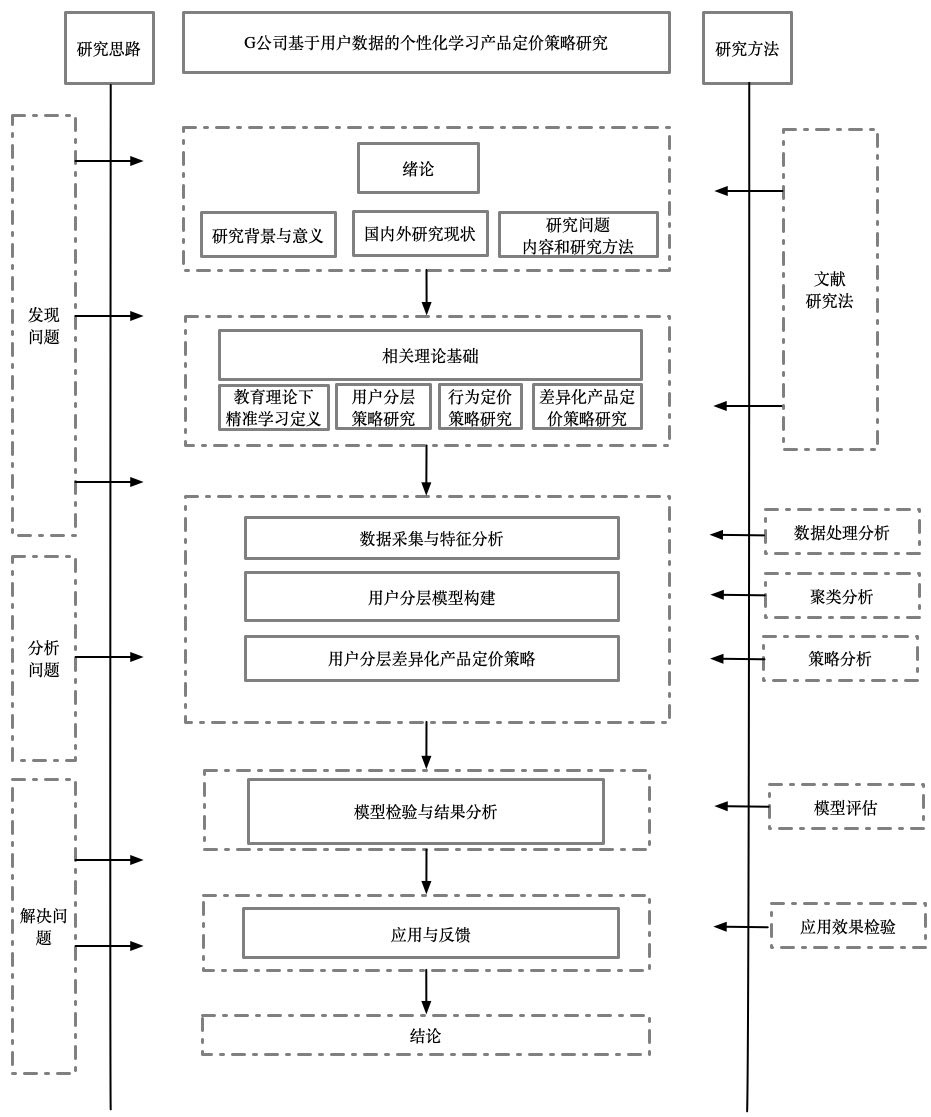
\includegraphics[width=0.8\textwidth]{figure/技术路线图.jpg}
    \caption{本研究的技术路线图}
    \label{fig:tech_route}
\end{figure}

首先在发现问题阶段,通过文献分析法梳理国家政策、教育市场趋势以及个性化学习与差异化定价策略的理论成果,明确当前智能教育产品中定价机制缺乏对学生个体差异、学习状态与支付意愿响应的问题,提出本研究的核心问题与研究思路。

接着在分析问题阶段,从理论与方法层面构建研究框架,界定学习画像特征提取、知识掌握状态分析、支付意愿特征分析与差异化组合定价策略设计的基本思路和实现路径;随后基于点阵笔采集的学习行为数据开展数据处理与特征提取,完成学习画像构建、知识掌握状态分析与支付意愿特征分析,形成差异化组合定价策略设计逻辑。

在解决问题阶段,完成差异化组合定价策略优化的设计与实现,构建端到端优化流程;并通过策略评估方法在实际数据上进行测试,检验组合推荐策略在用户转化率、平台收益与用户满意度等方面的综合表现,结合反馈不断优化学习画像特征提取方法与策略设计逻辑,提升策略效果与实用性。


\section{研究创新}

本研究面向初中数学场景下的教育智能硬件产品,以用户行为数据为基础,构建了一个面向知识点维度、服务内容组合和支付意愿差异的个性化定价模型。相较于传统教育产品的静态定价方式,本研究提出的动态组合式定价方法在理论建模、策略优化与商业应用层面均具有以下创新点:

\begin{itemize}
  \item \textbf{基于行为数据构建多维用户画像,实现行为驱动的动态分群与学习特征刻画。}  
  本研究在G公司智能点阵笔行为数据基础上,提取学习节奏、书写稳定性、题目跳过率、重做次数等多维特征,构建用户学习行为画像。通过K-Means聚类方法,实现了对用户在活跃度、稳定性、行为节奏等维度的自适应划分,替代传统基于静态成绩的用户划分方法,提升了用户价值建模的行为敏感性与时效性。

  \item \textbf{构建了面向知识点的掌握状态量化模型,支撑差异化资源分配与产品策略匹配。}  
  针对初中数学课程中多个核心知识点,设计了一套基于答题正确率、重做率、停顿时长等行为指标的知识点掌握度建模方法。该模型可针对每个用户精细化识别其掌握盲点,为后续产品策略(如推荐哪类教辅资源、引入何种服务)提供基础依据,提升了教育资源分配的精准性。

  \item \textbf{提出了结合用户行为分群与知识掌握状态的个性化服务组合推荐机制。}  
  本研究将用户分群信息与知识点掌握状态共同纳入定价决策机制,根据用户当前掌握情况与行为画像,推荐适配的教辅服务组合(如AI答疑、错题视频讲解、真人1V1答疑等),并考虑不同服务在不同知识点下的价值权重,构建差异化组合策略。这种机制突破了单一服务或定价等级的限制,实现了“用户-知识点-服务”三维匹配的策略设计。

  \item \textbf{构建了基于支付意愿概率的服务定价优化模型,实现收益最大化与策略可解释性的统一。}  
  在定价优化阶段,引入逻辑回归模型对用户支付意愿进行建模,融合用户特征、知识点掌握度与价格敏感度信息,计算不同组合方案下的支付概率。进而在控制服务成本与价格弹性的前提下,求解期望收益最大化的定价策略,形成端到端的个性化定价优化流程,兼顾商业目标与用户接受度。

  \item \textbf{提出了可扩展的组合定价建模框架,具有较强的跨平台与跨学科适应能力。}  
  本研究所提出的“学习行为—知识掌握—支付意愿—组合定价”建模路径,具有较强的模块解耦能力与策略可扩展性。除初中数学场景外,该模型亦可迁移至其他具备行为记录能力的学科或平台(如英语听说系统、科学探究平台等),为后续智能教育产品提供定价机制的通用范式。
\end{itemize}

\section{论文章节}

本文围绕基于学习行为数据的教育产品定价问题,在深入分析个性化教育发展背景及教育科技产品实际应用需求的基础上,结合用户分群建模、学习潜力预测与动态定价机制设计等方法,构建了数据驱动的教育产品定价策略体系,并开展实证验证与策略评估。全文结构安排如下:

第一章 绪论:介绍本研究的背景与意义,说明研究主旨与目标,明确研究内容与方法,回顾国内外相关研究现状,提出本研究的技术路线与论文总体结构。

第二章 理论基础与相关方法:系统阐述个性化教育、行为定价、用户分群与策略建模等相关理论基础,结合聚类分析、行为建模与定价优化等关键技术手段,构建论文研究的理论支撑体系。

第三章 研究内容与技术方法:围绕“发现问题—分析问题—解决问题”的研究主线,详细说明数据采集、特征建模、用户聚类、策略设计与模型评估等研究环节,建立完整的策略构建流程,并结合实际教育数据开展实验建模。

第四章 实证验证与策略评估:基于用户行为数据与平台反馈数据,开展定价策略的效果测试,评估其在提升平台收益、用户接受率与个性化服务水平等方面的表现,验证模型的稳定性、适应性与可推广性。

第五章 研究总结与未来展望:总结本文的主要研究成果与理论贡献,分析当前研究的限制与不足,探讨本研究在更大规模教育平台场景中的扩展潜力,并展望未来行为定价策略在教育智能化发展中的研究前景。


% \begin{itemize}
%   \item 参考文献的录入请参考\ref{sec:relatedwork:ref};
%   \item 图片插入参考\ref{sec:relatedwork:table};
%   \item 分数和公式参考\ref{sec:relatedwork:equation};
%   \item Latex绘图工具参考\ref{sec:method:tikz};
%   \item 代码块参考\ref{sec:method:code};
% \end{itemize}
% !TeX root = ../main.tex
% -*- coding: utf-8 -*-

\chapter{相关理论基础}
\label{chapter:相关理论基础}

\section{个性化教育理论基础}
\label{sec:个性化教育理论基础}

在前文绪论部分已指出,随着“以学生为中心”的教育理念持续深化,个性化教育已成为推动教育公平、提高学习效率的重要方向。为了更好地理解本研究中“基于学习行为数据的用户分群与个性化定价策略”的理论基础,有必要首先对个性化教育的定义、理论渊源与技术路径进行系统梳理。

\subsection{个性化教育的定义}
个性化教育(Personalized Education)是指根据学生的兴趣、能力、学习习惯和发展需求,制定差异化的教学目标、内容与路径,以实现“因材施教”的教育目的。根据\cite{oecd2018teachers}的定义,个性化学习强调“在教育内容与教学方式上进行灵活调整,使每一位学生都能获得最大的发展机会”。

在中国教育部发布的《关于深化教育教学改革全面提高义务教育质量的意见》中亦明确指出,要“尊重学生个体差异,推进个性化教学和精准教学实践”,推动从“以教师为中心”向“以学生为中心”转型。

\subsection{个性化教育的理论基础}

个性化教育的基本理念强调以学习者为中心,根据学生的差异化特征提供定制化学习资源与支持。早期相关理论基础主要包括:

\begin{itemize}
\item 学习是个体在原有知识结构基础上主动建构意义的过程,建构主义学习理论由 \cite{piaget1971constructivism} 提出,强调尊重学生个体经验与认知方式差异;
\item 多元智能理论由 \cite{gardner1983frames}提出,指出个体智力表现具有语言、逻辑、空间、音乐、身体、自然、人际、自知等多维结构,教育应据此实施多通道输入与多样化反馈策略。
\end{itemize}

近年来,随着教育数据与智能技术的引入,个性化教育的理论体系逐渐拓展:

\begin{itemize}
\item 精准教学理论(Precision Teaching)由 \cite{kubina2012precision}提出,强调通过行为数据进行教学调整,采集学习过程数据并反馈于教学决策,是现代学习分析的前提;
\item 学习分析框架由 \cite{unesco2022analytics}提出,指出应基于学习者数据,理解与优化学习过程与环境,为个性化教育提供数据支撑;
\item 开放学习生态模型由 \cite{siemens2011openlearning}提出,认为个体在多源数据环境下需要推荐与引导机制支持;
\item 适应性学习路径理论由 \cite{chen2020adaptivepath}提出,基于学生知识图谱、能力水平与偏好模型,构建自适应学习路径系统,体现了个性化教育中“动态推送-实时反馈”的技术逻辑。
\end{itemize}

这些理论的共同特征是将“数据—模型—策略”作为个性化教育运行机制的基础,强调对学习行为的细粒度采集与建模,并以系统性设计支持差异化服务。

\subsection{个性化教育的实现路径}
随着教育信息化的发展,个性化教育逐步从理念转向系统实现。当前主流路径包括:

\begin{itemize}
\item 使用点阵笔、智能平板等终端实时采集书写行为数据,为建模提供基础;
\item 运用聚类分析、分类算法对用户行为建模,构建个体画像;
\item 基于画像推荐资源,实现教学策略的个性匹配。
\end{itemize}

在K12与在线教育等领域,个性化推荐与精准教学已成为实践方向,构成“数据—模型—反馈”的闭环路径。

\subsection*{小结}
个性化教育是本研究提出“用户画像—策略设计”逻辑路径的理论起点。通过回顾其演化、理论依据与技术路径,明确了本研究以用户行为为核心开展策略优化的逻辑基础。

\section{教育产品差异化定价与用户价值挖掘}
\label{sec:教育产品定价与价值建模}

尽管本研究以个性化教育为背景,但其研究核心并不在于教学内容或课程优化,而是聚焦教育科技产品作为市场商品的经济属性,尝试通过行为数据挖掘与策略建模实现差异化定价机制,从而提升资源配置效率与商业响应能力。为此,有必要从商品属性、定价理论与价值识别三个方面展开分析。

\subsection{教育产品的商品属性与定价动因}

教育类数字产品本质上是一种融合了“内容传递—服务支持—数据交互”的复合型数字商品,其使用效果强依赖用户的个体差异。与传统商品不同,教育产品的“价值实现”并非即刻可见,而需在持续使用、反馈优化的动态路径中才能体现,这使得其呈现出显著的“非均质消费”特征\cite{zhang2021educationalproduct}。

在实际运营中,用户的行为频次、学习稳定性、任务完成度等都可能影响产品的价值释放路径与感知体验,因此“统一定价”往往造成资源浪费或用户流失。Li and Wang (2020) 研究发现,平台用户参与路径存在明显的阶段性与波动性,若忽视这种动态异质性,极易导致策略失配和边际效益递减。

此外,随着在线教育平台对订阅制、功能解锁制、学段升级制等定价模型的探索,教育产品逐步转化为一种“基于行为的服务型商品”,价格不再仅反映内容成本或平均效用,而应体现用户实际表现与使用潜力(Yang \& Zhang, 2023)。因此,教育平台的定价机制需要具备“行为响应性”与“价值分层能力”。

\subsection{差异化定价的理论基础}

传统的定价机制主要建立在成本核算与市场均价的基础之上,但这类机制难以在用户个体价值高度分化的教育场景中发挥作用。Pigou (1920) 提出的差异化定价理论为该问题提供了理论支撑,指出若企业能基于用户支付意愿或效用预期进行价格划分,既可提升整体收益,也有助于不同群体获得匹配服务。

在教育产品场景中,差异化定价的本质在于通过行为数据识别用户的需求等级与使用潜力,并以此设定合理价格段位。Sun and Chen (2021) 基于MOOC平台实证发现,用户学习路径与价格弹性之间存在系统性关联,表明行为数据可用于价格分级模型的建立。这也意味着,教育平台可以通过识别“高潜力-高付费意愿”的用户群体,实施动态策略以提升整体转化效率。

\subsection{差异化定价建模路径}

为了将行为数据有效转化为定价依据,必须建立从行为识别、潜力分析到支付建模的完整差异化建模路径。该路径通常包括以下三个核心阶段,如图\ref{fig:user_value_model_flow}:

\begin{figure}[!h]
  \centering
  \begin{tikzpicture}[node distance=2cm, every node/.style={align=center, font=\small}, >=stealth]
    % 样式
    \tikzstyle{stage} = [rectangle, rounded corners, draw=black, fill=blue!10, minimum width=3.8cm, minimum height=1.4cm]
    \tikzstyle{output} = [rectangle, rounded corners, draw=black, fill=gray!20, minimum width=3.5cm, minimum height=1.2cm]
    \tikzstyle{arrow} = [thick,->]

    % 主体阶段节点
    \node[stage] (A) {用户行为建模\\User Segmentation};
    \node[stage, right of=A, xshift=3.5cm] (B) {学习潜力预测\\Learning Potential Prediction};
    \node[stage, right of=B, xshift=3.5cm] (C) {支付意愿建模\\Price Acceptance Modeling};

    % 输出节点
    \node[output, below of=B, yshift=-1.5cm] (D) {用于定价策略优化};

    % 箭头
    \draw[arrow] (A) -- (B);
    \draw[arrow] (B) -- (C);
    \draw[arrow] (B) -- (D);
  \end{tikzpicture}
  \caption{用户价值建模三阶段流程图}
  \label{fig:user_value_model_flow}
\end{figure}




首先,在用户行为建模阶段,需要通过数据聚类与行为特征分析方法对用户进行分层。Xu and Zhao (2019) 指出,用户在访问频率、活跃周期、操作稳定性等维度上呈现出显著异质性,通过K-means或密度聚类等算法可有效划分不同用户画像。这一阶段的目标是完成“用户个体差异识别”。

其次,学习潜力预测是价值建模的关键一环。\cite{he2020predicting} 研究表明,利用监督学习算法(如回归树、神经网络)可对用户的学习完成率、测评得分提升情况进行建模,从而评估其后续资源利用效率和平台贡献潜力。这一阶段聚焦“行为效能预测”,为后续定价提供量化输入。

最后,支付意愿建模环节则关注用户对价格变化的响应程度。\cite{choi2021priceacceptance}利用Logit模型刻画用户在不同价格设定下的选择概率分布,反映其对价格敏感度的异质性。同时,\cite{fader2005customerltv}所提出的生命周期价值模型(LTV)为平台在定价策略设计时提供了基于长期贡献视角的评估框架,有助于制定兼顾当前转化与长期留存的策略组合。

通过上述三阶段模型,教育平台可将用户行为数据逐步转化为价格决策信息,构建既具经济效率又具行为解释力的动态定价机制。

\subsection*{小结}

教育产品的定价问题不仅是市场策略问题,更是对“用户行为—使用价值—支付意愿”关系的建模问题。以差异化定价理论为基础,结合行为分群、效能预测与支付建模方法,平台可实现从“观察行为”到“调节价格”的策略闭环。本研究正是基于此逻辑,尝试构建一套面向真实用户行为数据的定价优化方案,以实现教育资源配置与平台收益的双重优化。
\section{用户分群理论基础}
\label{sec:用户分群理论}

在本研究的差异化组合定价策略设计中,用户分群是构建策略逻辑的重要基础环节。通过学习行为数据识别出在学习节奏、行为稳定性、知识掌握状态和资源使用偏好等方面存在结构性差异的用户群体,有助于提升定价策略的个性化精准度与商业应用效果。因此,有必要从用户分群理论的学理基础、方法依据及其在教育场景中的适配性等方面进行系统梳理。

\subsection{市场细分理论与行为分群基础}

用户分群(User Segmentation)理论最早源于市场营销领域。Kotler 在其《Marketing Management》一书中指出,市场细分的核心在于“在异质性市场中识别出内部同质、外部异质的消费者群体,以实现产品与价格策略的精准匹配”(\cite{kotler2016marketing})。这一理论为后续行为分析与个体价值挖掘提供了理论支撑,其基本假设包括:

\begin{itemize}
  \item 消费者之间存在可识别且有商业价值的系统性差异;
  \item 差异可以通过可量化特征表达;
  \item 充分利用差异有助于优化产品策略与价格策略,提升商业绩效。
\end{itemize}

随着平台型教育产品的兴起,市场细分理论进一步演化为行为分群(Behavioral Segmentation),强调通过用户在平台中的实际行为数据进行建模。与基于用户属性的静态分层不同,行为分群聚焦于用户在学习频率、答题路径、资源偏好等行为特征上的差异性,更适用于教育场景下高频互动与深度行为反馈的数据环境(\cite{xu2019usersegmentation})。

\subsection{用户分群方法概述}

在差异化定价策略设计中,用户分群不仅具备理论价值,在实际建模过程中也具有明确的可操作性。本研究采用 K-Means 聚类方法对用户行为画像特征进行分群建模,该方法具有实现简洁、收敛速度快、可解释性强等优点,广泛应用于教育数据挖掘与个性化推荐领域(\cite{sun2021moocpricing})。

K-Means 聚类算法通过最小化簇内平方误差(Within-Cluster Sum of Squares, WCSS)实现用户群体划分,其优化目标函数如下:

\begin{equation}
\mathcal{L}_{\text{KMeans}} = \sum_{i=1}^{K} \sum_{x_j \in C_i} \| x_j - \mu_i \|^2
\end{equation}

其中,$x_j$ 表示用户 $j$ 的学习行为特征向量,$\mu_i$ 表示第 $i$ 个簇的中心向量,$C_i$ 表示属于第 $i$ 个簇的用户集合。后续章节将对具体的特征变量设计与聚类建模过程进行详细展开。

\subsection{用户分群在差异化组合定价策略中的作用}

在本研究中,用户分群不仅是用户理解和用户画像构建的重要手段,更是支撑差异化组合定价策略设计的核心输入之一。分群结果可作用于以下三个层面:

\begin{itemize}
  \item \textbf{服务推荐策略的复杂度调节}:用户分群结果为不同群体的服务推荐结构和组合复杂度提供约束条件。例如,高活跃高接受意愿群体可推送高价值组合,低活跃群体则控制推荐服务数量和价格水平。
  \item \textbf{支付意愿建模中的调节变量}:分群标签作为行为-支付之间的桥梁,可提升支付意愿预测的准确性。已有研究(\cite{choi2021priceacceptance})表明,在用户价值建模中引入群体特征作为条件变量,有助于提升模型性能。
  \item \textbf{策略评估与分层分析依据}:分群结果为策略验证与收益分析提供分层标准,有助于衡量不同群体在资源接受度、定价接受率与产品转化效果方面的异质性表现。
\end{itemize}

\subsection{教育场景中的分群实践启示}

在教育场景中,学生群体在学习活跃度、行为稳定性、知识掌握路径、服务接受意愿等方面具有天然的异质性,通用定价模式无法精准适配不同用户的学习状态与资源需求。MOOC 平台与中小学智能学习平台的实践表明,通过行为特征构建用户分群,并据此开展差异化教学干预与产品推荐,可显著提升用户体验与平台收益(\cite{sun2021moocpricing})。

本研究借鉴上述实践经验,将用户分群作为差异化组合定价策略的重要组成部分,推动定价策略从传统静态规则向行为驱动的动态个性化机制演进。

\subsection*{小结}

本节从市场细分理论、行为分群方法和教育应用实践三个维度,系统梳理了用户分群理论的研究基础。用户分群作为差异化定价机制中的关键支撑,在服务推荐结构调节、支付意愿建模与策略评估分层中发挥重要作用。为后续知识点掌握状态分析、支付意愿刻画与组合策略设计提供理论基础与结构入口。

\section{知识点掌握状态建模理论}
\label{sec:知识点掌握状态建模理论}

在差异化组合定价策略设计中,知识点掌握状态建模是承接用户学习行为特征与服务推荐决策之间的重要环节。通过精准刻画学生在各知识点层面的掌握程度,能够为差异化服务组合设计提供细粒度依据,提升定价策略的个性化水平与资源分配效率。因此,有必要从知识点掌握状态建模的理论基础、方法体系与教育场景适配性等方面进行系统梳理。

\subsection{理论基础与研究启发}

知识点掌握状态建模(Mastery Modeling)起源于教育测量与学习分析(Learning Analytics)领域。其核心理念是通过学生的过程性学习数据,动态推断学生在各知识点上的掌握状态,为个性化教学、推荐系统及教育评估提供支持(\cite{siemens2011openlearning,chen2020adaptivepath})。

早期的知识掌握建模方法主要基于学习知识图谱(Learning Knowledge Graph, LKG),将学习内容结构化表示,并通过图谱节点的属性建模掌握程度(\cite{chen2020adaptivepath})。随着智能学习平台和在线教育环境的发展,过程性学习行为(如答题轨迹、学习时间、反馈行为等)被广泛应用于知识点掌握状态推断(\cite{sun2021moocpricing})。

此外,认知诊断模型(Cognitive Diagnostic Model, CDM)与贝叶斯知识追踪(Bayesian Knowledge Tracing, BKT)等方法也在个性化学习系统中广泛采用,为动态掌握状态建模提供了强有力的理论支持(\cite{delatorre_minchen_2014,corbett_anderson_1995})。

\subsection{建模逻辑与方法体系}

现有研究表明,知识点掌握状态建模主要包含以下几类建模思路:

\subsubsection{加权评分模型(Mastery Scoring Model)}

加权评分模型是当前智能学习平台中广泛应用的知识点掌握状态建模方法之一。该方法通过加权整合学生在学习过程中的多个行为特征,形成连续型掌握度评分(Mastery Score):

\begin{equation}
M_{ij} = \sum_{k=1}^{K} \alpha_k \cdot F_{ijk}
\end{equation}

其中,$M_{ij}$ 为学生 $i$ 在知识点 $j$ 上的掌握度评分,$F_{ijk}$ 为第 $k$ 个特征的量化指标,$\alpha_k$ 为特征加权系数。该方法具有实现简单、可解释性强的优点,广泛用于MOOC平台与K12智能学习产品(\cite{xu2019usersegmentation,sun2021moocpricing})。

\subsubsection{贝叶斯知识追踪模型(Bayesian Knowledge Tracing, BKT)}

BKT 是经典的概率图模型,广泛用于在线学习系统中动态追踪学生对知识点的掌握状态(\cite{corbett_anderson_1995})。BKT 将学生对某知识点的掌握状态建模为隐变量 $L_t$,并通过学生在不同时间步的答题表现更新掌握概率:

\begin{equation}
P(L_t | \text{history}) = \frac{P(C_t | L_t) P(L_{t-1})}{P(C_t)}
\end{equation}

其中 $P(L_t)$ 为时间 $t$ 对知识点的掌握概率,$C_t$ 为当前答题表现。BKT 可动态更新掌握状态,适用于需要实时反馈的智能教学场景。

\subsubsection{项目反应理论(Item Response Theory, IRT)}

IRT 是教育测量领域的经典模型,通过建立学生能力 $\theta_i$ 与题目难度 $b_j$、区分度 $a_j$ 等参数之间的关系,推断学生知识掌握水平(\cite{lord_1980}):

\begin{equation}
P_{ij} = \frac{1}{1 + \exp[-a_j(\theta_i - b_j)]}
\end{equation}

其中 $P_{ij}$ 为学生 $i$ 正确回答题目 $j$ 的概率,$\theta_i$ 作为学生整体能力指标亦可分解至知识点维度。IRT 为掌握状态建模提供了强有力的统计推断基础,近年来也被广泛集成至在线学习平台。

\subsubsection{学习曲线建模(Learning Curve Modeling)}

学习曲线建模通过追踪学生在特定知识点上的学习进展,拟合其掌握水平随时间变化趋势,典型模型形式为幂律学习曲线(Power Law of Learning):

\begin{equation}
Performance(t) = a \cdot t^{-b} + c
\end{equation}

其中 $t$ 为学习次数,$a, b, c$ 为拟合参数。学习曲线建模强调学习动态过程,适用于个性化推荐与服务优化策略设计(Newell \& Rosenbloom, 1981)。

\subsection{知识点掌握状态对差异化定价策略的作用}

知识点掌握状态建模结果可为差异化组合定价策略设计提供以下支持:

\begin{itemize}
  \item \textbf{服务内容推荐依据}:根据学生对不同知识点的掌握状态,动态推荐适配的服务组合,提升推荐效果与用户体验;
  \item \textbf{组合复杂度调节依据}:根据掌握薄弱程度设计不同复杂度的服务组合,提升资源配置效率;
  \item \textbf{支付意愿模型输入特征}:学生在薄弱知识点上的学习需求强烈,掌握状态作为支付意愿预测模型中的关键特征,有助于优化价格接受度预测效果。
\end{itemize}

已有研究(\cite{sun2021moocpricing,xu2019usersegmentation})指出,知识点掌握状态作为教育场景中的核心用户状态变量,能够有效提升差异化推荐与定价策略的优化能力,是智能教育平台实现高质量商业优化的重要支撑。

\subsection*{小结}

本节围绕知识点掌握状态建模的理论基础、典型建模方法与应用价值进行了系统梳理。掌握状态建模不仅在个性化教学中具有重要作用,也是差异化组合定价策略设计中的关键变量之一。通过引入行为驱动掌握建模、BKT、IRT 等多种方法理论,为后续支付意愿特征分析与组合定价优化提供了坚实的理论基础。


\section{行为定价理论基础}
\label{sec:行为定价理论}

行为定价(Behavior-based Pricing)是数字经济中个性化定价机制的一种核心理论,其强调通过用户在平台上的历史行为、使用轨迹与反馈表现,识别个体支付意愿的差异性,从而构建差异化的定价策略。与传统基于成本加成或均衡市场价格的定价方式不同,行为定价关注用户之间的响应异质性,强调“行为—效用—价格”之间的函数映射关系(\cite{chen2002consumer}),已广泛应用于电商推荐、平台激励与数字商品分层定价等场景。

\subsection{行为定价的理论渊源与经济学基础}

行为定价的理论基础可追溯至微观经济学中关于“价格歧视”(Price Discrimination)的研究框架。\cite{pigou1920economics}首次系统提出一级(完全歧视)、二级(版本歧视)、三级(群体歧视)三种形式,其中一级价格歧视即为企业能够精确了解个体支付意愿,并对不同消费者设定不同价格。

行为定价可视为一级与三级定价的融合路径,其不依赖消费者主观申报或精确身份识别,而是通过分析用户客观行为推断支付倾向,在兼顾隐私与公平性的同时实现收益最优化目标。

进一步地,\cite{ariely2003}提出的“coherent arbitrariness”理论指出,尽管个体支付决策带有一定随机性,但在自身行为基础上呈现出相对一致的支付模式,即行为具有稳定的心理锚定效应。这为基于用户行为构建价格预测模型提供了心理学与行为经济学的理论支持。

\subsection{行为变量与支付意愿的函数映射机制}

行为定价的核心机制在于建立一个从用户行为变量空间 $\mathcal{X}$ 到支付概率空间 $[0, 1]$ 的映射函数,即:

\begin{equation}
\Pr(y_i = 1 | x_i, p) = f(x_i, p)
\end{equation}

其中 $x_i$ 表示用户 $i$ 的历史行为特征向量,$p$ 为价格水平,$y_i \in {0, 1}$ 为是否支付的响应变量。函数 $f(\cdot)$ 可采用概率回归、树模型或神经网络实现,其本质是学习一个“行为—支付”间的响应函数。

在本研究中,平台的收益优化目标可表示为:

\begin{equation}
\max_{p} \ \Pi(p) = \sum_{i=1}^{n} \Pr(y_i = 1 | x_i, p) \cdot (p - c)
\end{equation}

其中 $c$ 为单位产品成本,$\Pi(p)$ 表示平台的期望利润函数。优化策略的关键在于设计合适的 $\Pr(\cdot)$ 函数,使其既具有行为解释力,又具备预测准确性。

\subsection{在教育平台中的实际演化路径}

在教育科技产品中,用户的学习轨迹、任务完成率、答题行为等数据为行为定价提供了良好的输入基础。\cite{zhang2021educationalproduct}指出,课程重读频率与夜间学习行为显著预测用户在付费环节的响应强度。\cite{sun2021moocpricing}通过聚类分析发现,MOOC 学习者可被划分为“稳步进阶型”“高频弃学型”“拖延波动型”等群体,其支付意愿呈现出明显的段差分布。

这一发现推动教育平台采用“滚动式行为定价”策略,即通过实时监测用户行为变化更新定价推荐,形成行为响应性价格体系。这种定价模式特别适用于平台订阅制、功能解锁型产品与定制服务包等教育产品形态。

\subsection{行为定价建模框架与优化函数}

本研究采用逻辑回归模型对用户支付概率进行建模,形式如下:

\begin{equation}
\Pr(y_i = 1 | x_i, p) = \frac{1}{1 + \exp(-(\beta_0 + \beta^\top x_i + \beta_p p))}
\end{equation}

其中,$\beta$ 表示行为特征权重,$\beta_p$ 表示价格敏感系数。该模型可通过最大似然估计获得参数,用于刻画个体行为与支付反应之间的交互效应。

为提升模型稳定性与策略鲁棒性,本文引入价格弹性正则项作为目标函数约束项,用以抑制因价格微调而引发支付概率剧烈波动的问题。最终优化目标函数为:

\begin{equation}
\mathcal{L} = -\sum_{i=1}^{n} \left[ y_i \log \hat{y}_i + (1 - y_i)\log(1 - \hat{y}_i) \right] + \lambda \cdot \left| \frac{\partial \hat{y}_i}{\partial p} \right|^2
\end{equation}

该正则项源自 \cite{choi2021priceacceptance}在电子商务定价中的策略控制方法,可提高模型的泛化能力与定价曲线的平滑性,避免策略波动引发用户流失。

\subsection*{小结}

行为定价理论为用户行为变量与支付意愿函数之间建立了系统映射机制,其本质是利用历史数据推断个体价值,并在定价决策中加以体现。作为本研究中支付建模的理论基础,本节所述方法为后续策略函数设计、最优价格求解与效益评估提供了结构化的理论支持。


\section{支付意愿建模理论}
\label{sec:支付意愿建模理论}

尽管行为定价强调“行为决定价格”,但在实际策略设计中,平台需要一个明确的函数模型将行为变量 $x_i$ 映射为用户对定价 $p$ 的响应概率 $\Pr(y_i=1|x_i,p)$。支付意愿建模(Willingness-to-Pay Modeling)正是完成这一映射的关键机制,决定了平台后续策略的可操作性、可解释性与优化空间。

\subsection{支付意愿的理论起点}

在传统消费者选择理论中,支付意愿被定义为个体对某一产品或服务的“主观边际效用达到价格水平”的阈值点(\cite{lancaster_1966})。随着行为经济学与信息技术的发展,研究者开始强调用户支付意愿的可预测性,即通过个体历史行为、社会属性与互动偏好建模其价格响应特征(\cite{louviere_et_al_2000})。

在平台场景中,支付意愿并非静态存在,而是受用户行为状态与外部价格刺激共同影响的动态函数。因此,建模用户支付概率 $\Pr(y_i = 1|x_i, p)$,不仅是对个体经济理性的刻画,更是平台收益函数构建与策略最优化的基础。

\subsection{概率建模路径:Logit 模型及其机制}

本研究采用逻辑回归(Logistic Regression)作为支付意愿的建模工具,其原因包括:

在预测任务中具有良好的可解释性;

能处理二分类问题;

可拓展到收益函数最优化任务中。

具体模型设定如下:

\begin{equation}
\Pr(y_i = 1 | x_i, p) = \frac{1}{1 + \exp(-(\beta_0 + \beta^\top x_i + \beta_p p))}
\label{eq:logit}
\end{equation}

其中:

$x_i$ 为用户的行为变量;

$p$ 为对应的价格水平;

$\beta$、$\beta_p$ 分别表示行为变量与价格对支付概率的边际影响。

该模型反映了“行为变量 + 价格刺激”共同决定用户支付概率的非线性结构,是行为定价逻辑的量化表达。

\subsection{对策略函数的支持作用}

如前所述,平台的收益函数可定义为:

\begin{equation}
\Pi(p) = \sum_{i=1}^{n} \Pr(y_i = 1 | x_i, p) \cdot (p - c)
\end{equation}

其中,$\Pr(y_i = 1 | x_i, p)$ 由公式 \eqref{eq:logit} 提供估计,$c$ 为产品单位成本。因此,支付意愿建模构成了收益最大化问题的目标函数输入。

更重要的是,通过对 $\beta_p$ 与 $\beta^\top x_i$ 的估计,平台可判断用户对价格的敏感性,进而构造行为响应函数与价格分段函数,实现个性化定价逻辑。

\subsection{正则项控制与模型稳定性}

在实际建模中,用户行为变量可能存在噪声,价格调整可能引发策略不稳定。为此,本研究在逻辑回归损失函数中引入价格敏感性正则项,以平滑支付概率曲线:

\begin{equation}
\mathcal{L} = -\sum_{i=1}^{n} \left[ y_i \log \hat{y}_i + (1 - y_i)\log(1 - \hat{y}_i) \right] + \lambda \cdot \left| \frac{\partial \hat{y}_i}{\partial p} \right|^2
\end{equation}

该正则项通过抑制模型对价格变化的极端响应,控制策略输出的稳定性,避免用户体验恶化与收益波动加剧。在电商场景中也采用类似方法验证其有效性。


\subsection*{小结}

支付意愿建模是连接行为变量与价格响应之间的核心机制,决定了平台能否实现从“观察行为”到“引导支付”的策略闭环。通过建立 $\Pr(y_i=1|x_i,p)$ 函数结构,平台可开展价格敏感性分析、个性化定价策略设计与收益优化仿真,为后续章节策略构建提供坚实建模基础。

\subsection{策略评估的理论基础}
\label{sec:策略评估理论}

个性化定价策略的有效性不仅取决于行为识别与支付意愿建模的准确性,更取决于所提出策略在收益提升、用户接受与模型稳定性方面的综合表现。因此,必须建立一套基于经济理论与管理科学的策略评估框架。

\cite{von_hippel_2005}指出,用户对平台机制的接受度往往基于其对价格调整的感知公平性与响应一致性。\cite{shugan_2004}亦强调,数据驱动策略若无系统评估机制,极易在收益函数最优与用户体验之间发生偏离。因此,策略评估必须同时满足以下三个目标:

\begin{itemize}
  \item \textbf{收益最优化}:平台收益是否提升;
  \item \textbf{用户接受性}:用户是否更倾向于完成支付;
  \item \textbf{输出稳定性}:策略结果在不同场景下是否稳健。
\end{itemize}

为量化以上目标,本文将引入以下核心理论指标作为评估工具,其定义如下:

\begin{itemize}
  \item \textbf{支付率(Purchase Rate)}:在定价策略下用户实际完成支付的比例:
  \begin{equation}
    \text{PurchaseRate} = \frac{1}{n} \sum_{i=1}^{n} \mathbb{I}(y_i = 1)
  \end{equation}
  其中,$\mathbb{I}(\cdot)$ 为指示函数,$y_i=1$ 表示用户 $i$ 成功支付。

  \item \textbf{人均收益(Revenue per User, RPU)}:策略实施后的平均收益水平:
  \begin{equation}
    \text{RPU} = \frac{1}{n} \sum_{i=1}^{n} y_i \cdot (p_i - c)
  \end{equation}
  其中,$p_i$ 为分配给用户 $i$ 的价格,$c$ 为产品边际成本。

  \item \textbf{价格弹性(Price Elasticity)}:反映用户支付概率对价格变动的敏感性:
  \begin{equation}
    \text{Elasticity}_i = \frac{\partial \Pr(y_i = 1 | x_i, p)}{\partial p}
  \end{equation}
  弹性值越大,说明用户对价格波动越敏感,策略鲁棒性越低。

\end{itemize}

上述指标将在后续实证章节中用于对不同定价策略的性能进行量化评估,为最终策略选择与推广提供理论依据与定量支撑。

\section*{本章小结}

本章从理论层面系统构建了“行为驱动的个性化定价”研究框架,为后续模型构建与实证分析奠定了理论基础。首先,回顾了个性化教育的发展背景与理论根源,明确了学习行为数据在教育资源精准配置中的核心作用。其次,从教育产品的经济属性出发,引入差异化定价与用户价值识别理论,界定了本研究的策略优化目标与理论依据。

\chapter{模型构建}
\label{chapter:模型构建}

上一章系统梳理了教育产品个性化定价的理论基础,明确了用户行为数据在推动教育产品价值识别与差异化定价中的关键作用。这些理论框架为建立面向教育场景的动态定价策略提供了方法指导。

本研究聚焦于G公司初三数学教育产品的差异化组合定价策略设计。与一般标准化教育产品不同,初三数学知识体系结构复杂,不同学生在知识点掌握程度、学习行为习惯以及支付能力等方面存在显著差异。同时,平台可提供的教辅服务模块(如视频讲解、真题练习、真人答疑、动态评测、学习系统使用时长)具备高度组合灵活性,产品定价空间较大。如何基于用户差异化特征,动态生成最优知识点-服务组合,并实现收益最大化,成为平台差异化定价策略设计的重要课题。

针对上述业务需求,本文设计了以用户行为分群、知识点掌握状态建模、支付意愿建模与差异化组合定价策略为核心环节的建模流程,形成端到端差异化组合定价优化框架,为平台个性化定价策略提供理论与方法支持。

本章后续将依次展开用户行为分群建模、知识点掌握状态建模、支付意愿建模与差异化组合定价策略模块的详细设计与建模过程描述。
\section{用户行为分群建模}
\label{sec:用户行为分群建模}

在初三数学教育产品定价实践中,平台用户在学习行为习惯、活跃度、稳定性及学习过程中的反馈表现等方面存在显著差异。若不区分用户行为差异,采用统一策略设计组合产品及定价,容易导致策略匹配度不足,影响整体收益表现及用户体验。因此,有必要在差异化组合定价策略过程中引入用户行为分群建模模块,基于用户行为特征,划分差异化用户群体,支撑后续策略空间约束及个性化组合推荐逻辑设计。

\subsection{分群建模目标}

本模块旨在通过学习行为特征分析,识别用户整体行为模式,生成用户分群标签 $g_i$,作为差异化组合定价策略过程中的关键输入变量之一,主要发挥以下作用:

\begin{itemize}
\item \textbf{策略空间约束}:根据用户行为分群结果,动态调整推荐组合复杂度及价格区间,提升策略匹配度;
\item \textbf{差异化策略引导}:不同用户群体关注点、学习时间有不同的差异,支付意愿差异明显,通过分群结果引导个性化策略设计;
\item \textbf{模型输入特征增强}:将分群标签作为支付意愿和定价策略建模输入特征之一,增强模型预测能力。
\end{itemize}

\subsection{行为特征设计}

为增强用户行为分群模型的业务解释性与应用价值,本文选取以下关键行为特征作为模型输入,形成用户学习行为特征向量 $x_j$:
\begin{itemize}
\item \textbf{avg\_daily\_learning\_time}:用户日均学习时长;
\item \textbf{skip\_rate}:跳题率,反映用户学习稳定性;
\item \textbf{pause\_count}:平均停顿次数,衡量思维犹豫程度;
\item \textbf{stroke\_count}:平均笔画数,反映操作复杂度;
\item \textbf{writing\_variability}:书写速度标准差,体现节奏稳定性;
\item \textbf{pen\_pressure\_avg}:书写压力均值,间接反映信心或焦虑状态。
\end{itemize}
上述特征均通过智能学习硬件与平台学习数据实时采集与处理,具有较高的数据质量与业务可解释性。行为特征向量 $x_j$ 将作为分群建模过程中的核心输入变量。

\subsection{分群建模方法}

本研究借鉴Sun and Chen(2021)在MOOC平台用户分群建模研究成果,采用K-Means聚类方法实现用户行为分群建模,模型具有简洁性、可解释性强、收敛快速等特点,适用于当前业务场景下高维连续行为特征空间建模需求。

K-Means模型目标为最小化簇内平方误差(Within-Cluster Sum of Squares, WCSS):

\begin{equation}
\mathcal{L}_{\text{KMeans}} = \sum_{i=1}^{K} \sum_{x_j \in C_i} \| x_j - \mu_i \|^2
\end{equation}

其中:

\begin{itemize}
\item $x_j$ 为用户 $j$ 的学习行为特征向量;
\item $\mu_i$ 为簇 $C_i$ 的质心向量;
\item $K$ 为预设聚类簇数;
\item $C_i$ 为第 $i$ 个簇对应的用户集合。
\end{itemize}

\subsection{分群建模结果}

分群建模结果以用户分群标签 $g_i$ 形式输入后续模块,标签取值为 $g_i \in \{A, B, C, D\}$,具体含义如下:

\begin{itemize}
  \item \textbf{A类—高活跃型}:日均学习时长长,跳题率低,行为频繁且持续稳定,反映出较高的学习投入与平台黏性;
  
  \item \textbf{B类—波动型}:学习行为不稳定,跳题率与停顿率较高,书写节奏波动大,表现出阶段性参与与任务执行不连贯的特征;
  
  \item \textbf{C类—低活跃型}:学习频次低,跳题率高,学习投入不足,行为特征稀疏,反映出低使用意愿或平台依赖度;
  
  \item \textbf{D类—高效率型}:操作节奏稳定、书写特征一致性强、平均答题时间短,虽整体学习时间不一定最长,但在单位时间内展现出较强的任务完成效率。
\end{itemize}


后续支付意愿建模模块与差异化组合定价策略模块将基于该分群标签 $g_i$ 引导策略空间设计,提升个性化策略匹配度与商业实用性。

\subsection*{小结}

本节围绕用户学习行为分群建模展开,基于K-Means聚类方法,利用用户学习过程中的关键行为特征,构建用户分群标签 $g_i$,为后续支付意愿建模与差异化组合定价策略提供重要输入特征,支撑个性化组合策略设计与收益优化目标实现。

\section{知识点掌握状态建模}
\label{sec:知识点掌握状态建模}

教育产品差异化组合定价策略设计需充分考虑用户在不同知识点层面的掌握差异,动态推荐针对性组合产品,提升定价策略匹配度与用户感知价值。因此,在差异化组合定价优化流程中,需构建知识点掌握状态建模模块,基于用户学习行为数据,判定用户当前阶段薄弱知识点集合 $Z_i$,支撑后续组合策略设计。

\subsection{建模目标}

本模块目标为基于用户学习行为特征,针对知识点粒度,计算用户对各知识点的掌握度得分 $M_{ij}$,并依据设定阈值判定薄弱知识点集合 $Z_i$,作为差异化组合定价策略模块的知识点输入变量。

\subsection{模型设计思路与引入}

在初三数学产品场景中,用户在同一知识点 $z_j$ 上的学习行为具有高度个体差异性:

\begin{itemize}
\item 用户在 $z_j$ 上完成的题目数量存在差异,且通常不会覆盖该知识点下所有题目;
\item 不同题目对知识点掌握度的贡献不同,核心题目(如高频考点题、典型解法题)对掌握度贡献更大,非核心题目影响相对较小;
\item 不同知识点对行为特征的敏感度不同,难度高的知识点(如数列)中长时间作答可能正常,简单知识点(如一元二次方程)中快速完成反映掌握更好。
\end{itemize}

若直接采用用户整体行为特征加权计算掌握度,容易忽略上述因素,导致掌握度判别不准确,影响后续组合策略设计。因此,本文设计分层建模策略:

\begin{itemize}
\item 在题目粒度 $q$ 上,融合用户在该题目上的行为特征,计算题目掌握评分 $S_{iqj}$;
\item 在知识点粒度 $z_j$ 上,按题目权重 $w_q$ 对题目掌握评分进行加权平均,计算用户对知识点的总体掌握度 $M_{ij}$。
\end{itemize}

例如,若用户在知识点“数列”上做了 $5$ 道题目,其中包含 $3$ 道核心题,$2$ 道非核心题,则该用户对“数列”的掌握度 $M_{ij}$ 应主要由核心题的掌握情况决定,非核心题贡献较小。同时,数列作为高难度知识点,其题目时间类特征在掌握度中权重应降低,以更真实反映掌握情况。

\subsection{行为特征设计}

知识点掌握状态建模需将用户学习过程行为特征映射至题目粒度,本文选取以下特征作为模型输入,特征计算均在题目粒度 $q$ 上进行:

\begin{itemize}
\item $c_{iqj}$:题目 $q$ 上用户 $i$ 的答题正确率(0 或 1);
\item $r_{iqj}$:题目 $q$ 上用户 $i$ 的重做次数(或重做标记);
\item $p_{iqj}$:题目 $q$ 上用户 $i$ 的平均停顿时间;
\item $t_{iqj}$:题目 $q$ 上用户 $i$ 的平均做题时间;
\item $s_{iqj}$:题目 $q$ 上用户 $i$ 是否跳题(跳题记为 1,完成记为 0)。
\end{itemize}

上述特征通过平台用户学习过程行为日志与智能学习硬件数据实时采集,具有良好的数据质量与业务解释性。

\subsection{题目掌握评分模型}

题目掌握评分 $S_{iqj}$ 采用加权Sigmoid融合模型,公式如下:

\begin{equation}
S_{iqj} = \sigma \left( \beta_1^{(z_j)} c_{iqj} + \beta_2^{(z_j)} r_{iqj} + \beta_3^{(z_j)} p_{iqj} + \beta_4^{(z_j)} t_{iqj} + \beta_5^{(z_j)} s_{iqj} \right)
\end{equation}

其中:

\begin{itemize}
\item $\beta_k^{(z_j)}$ 表示知识点 $z_j$ 对特征 $k$ 的敏感度系数,$k = 1, \ldots, 5$;
\item $\sigma(\cdot)$ 为Sigmoid归一化函数,$\sigma(x) = \frac{1}{1 + e^{-x}}$,将评分归一化至 $[0,1]$ 区间;
\item 评分 $S_{iqj}$ 反映用户在题目 $q$ 上的掌握水平,高分表示掌握良好,低分表示掌握薄弱。
\end{itemize}

\subsection{知识点掌握度计算}

用户 $i$ 对知识点 $z_j$ 的掌握度得分 $M_{ij}$ 计算公式如下:

\begin{equation}
M_{ij} = \frac{ \sum\limits_{q \in Q_{ij}} w_q \cdot S_{iqj} }{ \sum\limits_{q \in Q_{ij}} w_q }
\end{equation}

其中:

\begin{itemize}
\item $Q_{ij}$ 为用户 $i$ 在知识点 $z_j$ 下做过的题目集合;
\item $w_q$ 为题目 $q$ 的权重,核心题权重大,非核心题权重低,可依据知识点知识图谱和题目标签设定;
\item $S_{iqj}$ 为用户 $i$ 在题目 $q$ 上的掌握评分。
\end{itemize}

该设计可有效融合用户在知识点 $z_j$ 上不同题目的学习情况,动态反映掌握状态,解决了用户覆盖度不完整、题目价值差异、知识点行为敏感度差异等问题。

\subsection{薄弱知识点判别}

根据掌握度得分 $M_{ij}$,设定判别阈值 $\theta$,判定用户 $i$ 的薄弱知识点集合 $Z_i$:

\begin{equation}
Z_i = \{ z_j \mid M_{ij} < \theta \}
\end{equation}

其中 $\theta$ 可通过平台历史学习效果数据与专家经验共同设定。通常可设置为全平台 $M_{ij}$ 分布下的特定分位点(如25\%分位点),动态适应整体学习效果分布变化。

\subsection{建模结果应用}

薄弱知识点集合 $Z_i$ 将作为差异化组合定价策略模块的知识点输入,支撑个性化组合设计,提升策略匹配度与用户感知价值。后续差异化组合定价策略模块将基于 $Z_i$ 动态推荐知识点-服务组合,优化整体收益表现。

\subsection*{小结}

本节围绕知识点掌握状态建模展开,针对初三数学产品场景中用户学习行为的复杂性,设计了分层建模策略,先在题目粒度计算题目掌握评分 $S_{iqj}$,再在知识点粒度计算掌握度得分 $M_{ij}$,并判定薄弱知识点集合 $Z_i$,为后续差异化组合定价策略提供关键输入变量,增强策略个性化与匹配度。


\section{支付意愿建模}
\label{sec:支付意愿建模}

在差异化组合定价策略设计中,支付意愿建模是实现“行为—价值—价格”映射关系的关键环节。尽管用户行为分群模型已刻画出用户在学习行为与操作习惯上的差异性,但对于产品定价而言,更关键的是识别用户的付费能力与付费意愿,即预测用户在面对不同产品组合与价格区间时的潜在响应水平。

\subsection{建模目标与业务背景}

由于平台用户均已完成至少一次付费操作,传统意义上的“是否付费”标签不再适用。因此,本文关注的是用户在历史订单中表现出的\textbf{付费水平差异},并以此为基础,建立用户“支付意愿强度”预测模型。该模型的目标不仅是判断用户“是否支付”,而是量化其未来在个性化组合推荐中接受价格与服务强度的倾向性,用于后续差异化策略空间设计与收益最大化路径规划。

\subsection{输入特征设计}

本节模型主要依赖两个信息源:

\begin{itemize}
  \item \textbf{支付行为特征 $a_i$}:
  \begin{itemize}
    \item $a_i^{(1)}$:首次付费金额,反映初始支付门槛;
    \item $a_i^{\max}$:最大历史单笔付费金额,反映用户支付能力上限;
    \item $\bar{a}_i$:历史订单均值,反映总体支付预期;
    \item $o_i$:历史订单数量,反映用户对平台服务接受程度;
  \end{itemize}

  \item \textbf{行为分群标签 $g_i$}:
  \begin{itemize}
    \item A类:高活跃型;
    \item B类:中活跃型;
    \item C类:低活跃型;
    \item D类:高效稳定型。
  \end{itemize}
  分群标签体现了用户在学习行为上的类型归属,为支付意愿提供结构性调节因素。
\end{itemize}

\subsection{建模方法与数学表达}

为保持模型简洁与可解释性,本文采用Logit模型对支付意愿强度进行建模,其结构如下:

\begin{equation}
\Pr(y_i^{pay} = 1 | a_i, g_i) = \frac{1}{1 + \exp(-(\theta^\top a_i + \gamma_{g_i}))}
\end{equation}

其中:
\begin{itemize}
  \item $y_i^{pay}$ 表示用户 $i$ 是否具备高支付意愿(构建为标签或分段等级);
  \item $\theta$ 为支付行为特征的权重向量;
  \item $\gamma_{g_i}$ 为分群标签 $g_i$ 对整体支付意愿的调节偏置(如 One-hot 编码);
  \item 输出为支付概率,可视为未来支付能力的估计值。
\end{itemize}

为防止模型对某一价格段出现过度敏感的预测结果,进一步引入价格弹性正则项,以控制输出波动:

\begin{equation}
\mathcal{L} = -\sum_{i=1}^{n} \left[ y_i^{pay} \log \hat{y}_i + (1 - y_i^{pay}) \log(1 - \hat{y}_i) \right] + \lambda \cdot \left| \frac{\partial \hat{y}_i}{\partial p} \right|^2
\end{equation}

该正则项有助于维持支付预测函数对价格变化的稳定响应,从而提升策略平滑性与商业可接受度。

\subsection{模型结果的应用价值}

支付意愿预测结果 $\Pr(y_i^{pay} = 1)$ 将直接作为后续定价策略模块的控制输入,具体功能包括:

\begin{itemize}
  \item \textbf{推荐强度控制}:意愿高者可推荐更复杂、更高价值服务组合;
  \item \textbf{定价区间规划}:在收益最大化模型中参与最优价格搜索;
  \item \textbf{风险调控}:避免向低支付意愿用户推送高价组合,降低流失率。
\end{itemize}

\subsection*{小结}

本节从用户历史订单数据出发,设计了面向平台已有付费用户群体的支付意愿建模框架。模型依托支付行为特征与行为分群标签构建输入,采用Logit结构完成支付倾向建模,并为后续定价策略中的价格、服务等级与组合复杂度设计提供量化依据,实现策略层面的精准性与商业价值最大化。
\section{差异化组合定价策略}
\label{sec:差异化组合定价策略}

在完成用户行为分群、知识点掌握状态与支付意愿建模的基础上,平台需依据个体用户的差异化学习需求与支付能力,制定具有针对性的知识点-服务-时长推荐组合,并在此基础上设置合理价格,最终实现平台整体收益的最优化。本节将该问题拆解为两个核心子任务:\textbf{(1)个体定价策略构建}与\textbf{(2)平台收益优化模型设计},分别阐述推荐组合的生成逻辑与收益函数构建原理。

\subsection{个体推荐组合与定价机制设计}
\label{sec:sub_定价策略设计}

\subsubsection*{(一)组合策略的构成单位}

本研究中推荐的定价对象并非单一服务或题目,而是用户 $i$ 在其薄弱知识点 $z_j$ 下的定制化服务包组合,其构成单位为三元组 $(z_j, s_k, \tau_{ijk})$,即:

\begin{itemize}
\item $z_j$:上文模型构建的薄弱知识点集合;
\item $v_{jk}$:产品服务贡献值,如产品类型(如 1V1 答疑、视频讲解等)每个单位时长价值;
\item $\tau_{ijk}$:该服务在该知识点下的推荐服务时长(单位为分钟数或课时数),由后续公式动态计算。
\end{itemize}

多个三元组构成完整的用户组合推荐策略,记为:

\begin{equation}
combo_i = \left\{ (z_j, v_{jk}, \tau_{ijk}) \mid z_j \in Z_i, v_{jk} \in \mathcal{V} \right\}
\end{equation}

其中 $Z_i$ 表示用户的薄弱知识点集合,$\mathcal{v}$ 表示平台支持的服务价值贡献集合。

\subsubsection*{(二)服务价值贡献}

平台提供的服务类型($s_k$)按照个性化程度与交付成本分为五个等级,见表~\ref{tab:service_level_summary}。不同服务在不同知识点下的服务价值贡献 $v_{jk}$(即单位时长带来的平台预期收益)是推荐定价建模中的核心输入变量。

\begin{table}[!h]
\centering
\caption{服务等级说明}
\begin{tabular}{c c c}
\toprule
服务等级 & 类型 & 特点说明 \\
\midrule
等级1 & 1V1实时答疑 & 高度定制,实时交互,教学资源密集,单价最高 \\
等级2 & 真人答疑 & 延迟响应,有答复保障,人工参与 \\
等级3 & 视频讲解 & 标准内容,适合通识训练,资源固定 \\
等级4 & AI错题巩固 & 自动任务,高效率,反馈可控 \\
等级5 & AI答疑 & 模板响应,低成本,适合入门问题 \\
\bottomrule
\end{tabular}
\label{tab:service_level_summary}
\end{table}

\vspace{0.5em}
服务价值贡献 $v_{jk}$ 并非直接对应用户价格,而是平台根据历史收益、服务成本与教学难度等因素推算出的单位时长价值潜力指标。该指标用于后续收益计算与推荐策略排序。

平台在设定 $v_{jk}$ 时,综合考虑以下三类因素:

\begin{itemize}
\item \textbf{(1)知识点难度系数 $\alpha_j$}:来源于平台知识图谱中知识点 $z_j$ 的标注难度等级,难度越高,学习资源配置应越丰富;
\item \textbf{(2)服务等级成本系数 $\beta_k$}:体现服务 $s_k$ 在单位时间内的资源投入强度,例如1V1答疑的人力排班成本远高于AI答疑;
\item \textbf{(3)历史业务表现系数 $\gamma_{jk}$}:以该服务在该知识点下的历史用户转化率、满意度、续购率等业务指标进行回归打分。
\end{itemize}

为实现量化建模,平台构建如下加权组合函数用于评估单位价值贡献:

\begin{equation}
v_{jk} = w_1 \cdot \alpha_j + w_2 \cdot \beta_k + w_3 \cdot \gamma_{jk}
\end{equation}

其中:

$w_1, w_2, w_3$ 为人工调参设定的全局权重(满足 $w_1 + w_2 + w_3 = 1$),初始由教育产品专家经验设定,后续结合 A/B 实验自动调整;
$\alpha_j$ 为知识点 $z_j$ 的难度等级(如按1-5标定并归一化);
$\beta_k$ 为服务 $s_k$ 的单位时长交付成本(归一化);
$\gamma_{jk}$ 为历史运营数据中该服务-知识点组合的加权表现值。


\vspace{0.5em}
最终得到如下归一化示意矩阵(示意为比例值):

\begin{table}[!h]
\centering
\caption{知识点-服务等级单位时间价值贡献示意矩阵(归一化比例制)}
\begin{tabular}{c c c c c c}
\toprule
知识点 / 服务等级 & 1V1实时答疑 & 真人答疑 & 视频讲解 & AI错题巩固 & AI答疑 \\
\midrule
数列 & 1.00 & 0.50 & 0.20 & 0.10 & 0.05 \\
几何 & 1.00 & 0.50 & 0.20 & 0.10 & 0.05 \\
二次函数 & 0.80 & 0.40 & 0.20 & 0.10 & 0.07 \\
一次方程 & 0.60 & 0.30 & 0.15 & 0.10 & 0.08 \\
实数根式 & 0.40 & 0.20 & 0.10 & 0.12 & 0.10 \\
\bottomrule
\end{tabular}
\label{tab:value_contribution_matrix}
\end{table}

\vspace{0.5em}
上述矩阵不仅体现了平台对不同教学场景的服务结构评估逻辑,也为后续推荐组合 $combo_i$ 的收益估计与策略排序提供基础依据,是整套定价机制中最核心的策略输入之一。



\subsubsection*{(三)推荐服务时长的计算逻辑}

推荐服务时长 $\tau_{ijk}$ 是三元组 $(z_j, s_k, \tau_{ijk})$ 的核心组成部分,决定了平台为每位用户提供服务的深度。本文采用以下计算公式:

\begin{equation}
\tau_{ijk} = \eta \cdot (1 - M_{ij}) \cdot \kappa(g_i) \cdot \Pr(y_i = 1)
\end{equation}

其中:

\begin{itemize}
\item $M_{ij}$:用户 $i$ 对知识点 $z_j$ 的掌握度;
\item $\kappa(g_i)$:用户行为分群 $g_i$ 对推荐强度的调节系数;
\item $\Pr(y_i = 1)$:用户对教育产品的支付意愿预测概率;
\item $\eta$:全局单位服务时长基准(如30分钟)。
\end{itemize}

该设计实现了以下策略逻辑:
掌握度低 → 推荐更多时间;
用户活跃度低 → 推荐时长适度放大;
支付意愿高 → 推荐配置向上增强,体现转化潜力。

\subsubsection*{(四)个体推荐组合价格估计}

平台在计算个体推荐价格时,引入统一的单位服务时间定价基准 $\phi$(例如 $\phi = 5$ 元/分钟),并结合服务价值贡献 $v_{jk}$ 与推荐时长 $\tau_{ijk}$,计算理论定价贡献 $r_{ijk}$:

\begin{equation}
r_{ijk} = \phi \cdot \tau_{ijk} \cdot v_{jk}
\end{equation}

最终,用户 $i$ 的推荐组合整体定价为:

\begin{equation}
R_i = \sum_{(z_j, s_k) \in combo_i} r_{ijk} = \phi \cdot \sum_{(z_j, s_k)} \tau_{ijk} \cdot v_{jk}
\end{equation}

其中:

$\phi$ 为单位时间定价基准,由平台统一设定;

$v_{jk}$ 为服务 $s_k$ 在知识点 $z_j$ 上的单位价值;

$\tau_{ijk}$ 为推荐时长。

该定价机制可实现价格动态联动:在推荐时长、服务类型或价值贡献变化时自动调整总定价。同时定价结果也具备良好的结构可解释性,有利于后续组合的结构优化与迭代推荐。

\subsubsection*{(五)组合推荐示意表}

为增强理解,以下表格展示了平台基于定价基准 $\phi = 5$(单位:元/分钟),结合用户行为与掌握状态,为用户 $i$ 生成的个性化推荐组合策略:

\begin{table}[!h]
\centering
\caption{用户 $i$ 推荐组合策略示例}
\begin{tabular}{c c c c c}
\toprule
知识点 $z_j$ & 服务类型 $s_k$ & 推荐时长 $\tau_{ijk}$(分钟) & 单位价值 $v_{jk}$ & 推荐价值 $r_{ijk}$(元) \\
\midrule
数列 & 1V1实时答疑 & 60 & 1.00 & 300.00 \\
几何 & 真人答疑 & 45 & 0.50 & 112.50 \\
二次函数 & 视频讲解 & 30 & 0.20 & 30.00 \\
一次方程 & AI错题巩固 & 20 & 0.10 & 10.00 \\
\bottomrule
\end{tabular}
\label{tab:combo_example}
\end{table}

推荐组合的总定价为:

\begin{equation}
R_i = \phi \cdot \sum_{(z_j, s_k)} \tau_{ijk} \cdot v_{jk} = 5 \cdot (60 \cdot 1.00 + 45 \cdot 0.50 + 30 \cdot 0.20 + 20 \cdot 0.10) = 452.5 \ \text{元}
\end{equation}

该定价代表平台依据用户特征所推荐服务组合的理论价值估计,并将作为后续收益函数优化的重要输入变量。

\subsection{平台收益最大化优化模型}
\label{sec:sub_收益最大化}

在获得所有用户推荐组合的理论价值估计 $R_i$ 后,平台需要在价格制定和资源分配约束下,优化整体收益函数 $\Pi$。

\subsubsection*{(一)收益函数构建}

在构建平台收益函数时,需明确每项推荐组合的交付成本构成。由于服务等级差异巨大(如1V1需人工,AI服务几乎为零边际成本),平台为各等级服务定义了单位时长成本比例 $q_k$,以对应其对整体收益的影响。示意如下:

\begin{table}[!h]
\centering
\caption{服务等级单位时长成本比例设定}
\begin{tabular}{c c c}
\toprule
服务等级 & 服务类型 & 成本比例 $q_k$(占定价比例) \\
\midrule
等级1 & 1V1实时答疑 & 40\% \\
等级2 & 真人答疑 & 30\% \\
等级3 & 视频讲解 & 15\% \\
等级4 & AI错题巩固 & 8\% \\
等级5 & AI答疑 & 3\% \\
\bottomrule
\end{tabular}
\label{tab:cost_ratio_table}
\end{table}

基于此,用户 $i$ 的推荐组合交付成本 $C_i$ 可估算为:

\begin{equation}
C_i = \sum_{(z_j, s_k)} r_{ijk} \cdot q_k
\end{equation}

进而,平台整体预期收益函数为:

\begin{equation}
\Pi = \sum_{i=1}^{N} f_{\text{pay}}(a_i, g_i) \cdot (R_i - C_i)
\end{equation}

其中:

$f_{\text{pay}}(a_i, g_i)$ 为上一节支付意愿预测模型输出;

$R_i$ 为平台对用户推荐组合的定价估计;

$C_i$ 为服务交付成本,动态与组合结构、时长和服务等级相关。

该模型设计明确将“收益 = 价格 - 成本”机制引入差异化定价策略中,兼顾服务层次差异与个体推荐弹性,为收益最大化策略提供了结构性支持。


\subsubsection*{(二)模型优化意义}

该收益函数兼顾用户行为特征、知识点掌握状态与支付意愿响应能力,实现以下建模目的:

\begin{itemize}
\item 利用分群标签与掌握状态控制推荐强度,体现用户画像驱动;
\item 利用支付意愿预测结果进行价格容忍区间调整,防止过度推高导致流失;
\item 服务等级与推荐时长共同决定成本和效益,确保组合结构合理。
\end{itemize}

\subsubsection*{(三)策略输出应用}

通过对 $\Pi$ 的最优化求解,平台可得到每一位用户的个性化推荐定价方案与最大收益预估,并进一步用于:

\begin{itemize}
\item 教辅资源调度计划(如教师分配、AI服务调用);
\item 市场营销场景下的优惠券策略与价格推荐;
\item 用户续购、二次销售的策略嵌套设计。
\end{itemize}

\subsection*{小结}

本节围绕“用户服务组合推荐—推荐价格估计—平台收益函数优化”的链式结构,系统构建了一个兼顾用户行为、学习水平与支付能力的智能定价机制。通过组合三元组 $(z_j, v_{jk}, \tau_{ijk})$ 的结构性设计,平台可实现产品定价的精细控制与用户体验的精准匹配,为个性化教育服务在智能化运营层面提供可部署的建模基础。



% \section{差异化组合定价策略}
% \label{sec:差异化组合定价策略}

% 在完成用户行为分群建模、知识点掌握状态建模与支付意愿建模之后,差异化组合定价策略模块以用户薄弱知识点集合 $Z_i$、用户支付意愿预测 $\Pr(y_i=1|x_i,g_i,p)$ 以及分群标签 $g_i$ 为输入,优化生成用户个性化知识点-服务组合推荐策略 $combo_i$,实现收益最大化目标。


% \subsection{优化建模目标}

% 差异化组合定价策略的核心目标是根据用户差异化特征动态生成个性化组合推荐策略 $combo_i$,实现以下优化目标:

% \begin{itemize}
% \item \textbf{收益最大化}:最大化用户在推荐组合下的期望收益;
% \item \textbf{策略匹配度提升}:根据用户知识点掌握状态,精准定位推荐知识点;
% \item \textbf{策略复杂度控制}:根据用户分群标签与支付意愿,动态调整推荐组合复杂度与服务等级,提升策略可接受性与用户体验。
% \end{itemize}

% \subsection{知识点优选}

% 虽然知识点掌握状态建模模块已输出用户薄弱知识点集合 $Z_i$,但在实际组合定价策略中,不宜直接推送全部 $Z_i$,否则会导致推荐内容过重,用户认知负担大,转化效果不佳。因此,需对 $Z_i$ 进行优选,筛选出优先推荐知识点子集 $\hat{Z}_i \subseteq Z_i$,作为最终推荐知识点集合。

% 优选逻辑包括以下因素:

% \begin{itemize}
% \item \textbf{掌握度优先性}:优先推荐掌握度 $M_{ij}$ 较低的知识点;
% \item \textbf{服务价值优先性}:优先推荐对应服务价值贡献较高的知识点;
% \item \textbf{组合复杂度控制}:根据 $\Pr(y_i=1)$ 和 $g_i$ 控制 $\hat{Z}_i$ 的推荐规模,意愿高可推荐更多知识点,意愿低则控制数量。
% \end{itemize}

% 整体可设计知识点优选排序得分:

% \begin{equation}
% score_{ij} = -M_{ij} + \rho \cdot \sum_{k} v_{jk}
% \end{equation}

% 其中 $\rho$ 为价值贡献权重系数,排序后选取Top-N个知识点组成 $\hat{Z}_i$,$N$动态调整:

% \begin{equation}
% N_i = \delta(g_i) \cdot \Pr(y_i=1|x_i,g_i,p)
% \end{equation}

% 其中 $\delta(g_i)$ 为不同分群标签对应的基础知识点推荐规模系数。

% \subsection{服务模块等级匹配设计}

% 根据平台实际业务,服务模块按价值等级可划分为以下五类,从高到低分别为:

% \begin{itemize}
% \item \textbf{等级1:1V1实时答疑};
% \item \textbf{等级2:真人答疑};
% \item \textbf{等级3:视频讲解};
% \item \textbf{等级4:AI错题巩固};
% \item \textbf{等级5:AI答疑}。
% \end{itemize}

% 每个知识点 $z_j$ 下可配置若干服务等级模块,组合策略过程中需根据用户支付意愿 $\Pr(y_i=1)$ 动态调整推荐服务等级:

% \begin{itemize}
% \item 高支付意愿用户:优先推荐高价值服务(等级1-3),可搭配等级4-5服务;
% \item 中等支付意愿用户:以等级3-4服务为主,辅以少量高价值服务;
% \item 低支付意愿用户:以等级4-5轻量服务为主,控制组合成本。
% \end{itemize}

% 整体组合复杂度控制策略为:

% \begin{equation}
% L_i = \kappa(g_i) \cdot \Pr(y_i=1|x_i,g_i,p)
% \end{equation}

% 其中 $L_i$ 为推荐服务等级配置深度,$\kappa(g_i)$ 为不同分群标签对应的基础服务等级配置系数。

% \subsection{教辅服务价值建模}

% 平台为不同知识点-服务等级组合预设价值贡献矩阵 $v_{jk}^{(l)}$,其中 $v_{jk}^{(l)}$ 表示知识点 $z_j$ 下服务等级 $l$ 对应服务模块的价值贡献。

% \textbf{业务定价逻辑说明}:

% 平台在实际业务中,教辅服务价值贡献设计不仅考虑服务本身的价值等级,还需结合知识点难度特性:

% \begin{itemize}
% \item 难度高的知识点(如数列、几何)对教学资源需求更高,用户付费意愿更强,且高阶服务(如1V1、真人答疑)交付成本更高 → 在价值贡献矩阵中体现出更高占比;
% \item 简单知识点(如实数、根式计算)教学资源需求相对较低,AI类服务更具性价比 → 高阶服务价值贡献占比较低,AI服务贡献占比较高;
% \item 平台定价策略综合考虑\textbf{用户价值感知}与\textbf{服务交付成本},使得价值贡献矩阵符合商业逻辑与用户体验。
% \end{itemize}

% 示意表如下(按比例展示,非真实价格):

% \begin{table}[!h]
% \centering
% \caption{知识点-服务等级价值贡献示意表(按比例)}
% \begin{tabular}{c c c c c c}
% \toprule
% 知识点 / 服务等级 & 1V1实时答疑 & 真人答疑 & 视频讲解 & AI错题巩固 & AI答疑 \\
% \midrule
% 数列 & 1.00 & 0.50 & 0.20 & 0.10 & 0.05 \\
% 几何 & 1.00 & 0.50 & 0.20 & 0.10 & 0.05 \\
% 二次函数 & 0.80 & 0.40 & 0.20 & 0.10 & 0.07 \\
% 一次方程应用题 & 0.60 & 0.30 & 0.15 & 0.10 & 0.08 \\
% 实数、根式计算 & 0.40 & 0.20 & 0.10 & 0.12 & 0.10 \\
% \bottomrule
% \end{tabular}
% \label{tab:knowledge_service_value}
% \end{table}

% 上述价值矩阵 $v_{jk}^{(l)}$ 为策略提供价值约束依据,影响组合收益计算与推荐排序。

% \subsection{收益最大化模型}

% 最终,差异化组合定价策略模型目标为收益最大化,优化目标函数如下:

% \begin{equation}
% \max_{combo_i} \ \Pi = \sum_{i=1}^{N} \Pr(y_i=1|x_i,g_i,p) \cdot \left( \sum_{(z_j, s_k^{(l)}) \in combo_i} v_{jk}^{(l)} - c_{combo_i} \right)
% \end{equation}

% 其中:

% \begin{itemize}
% \item $N$ 为平台用户总数;
% \item $combo_i$ 为用户 $i$ 推荐的知识点-服务等级组合;
% \item $v_{jk}^{(l)}$ 为知识点-服务等级价值贡献;
% \item $c_{combo_i}$ 为组合 $combo_i$ 的整体成本;
% \item $\Pr(y_i=1|x_i,g_i,p)$ 为用户 $i$ 对当前组合的支付意愿预测;
% \item $\Pi$ 为平台整体收益目标。
% \end{itemize}

% 优化过程中,需在收益最大化与策略复杂度、用户体验之间实现平衡,确保推荐组合策略具备商业可用性与用户接受度。

% \subsection*{小结}

% 本节围绕差异化组合定价策略展开,基于用户薄弱知识点集合 $Z_i$,筛选优选推荐子集 $\hat{Z}_i$,根据支付意愿 $\Pr(y_i=1)$ 和分群标签 $g_i$ 动态调整服务等级推荐,优化生成用户个性化知识点-服务组合推荐策略 $combo_i$,实现收益最大化目标,为平台差异化定价策略提供核心优化机制。



\section{端到端差异化组合定价流程框架}
\label{sec:端到端组合定价优化流程}

在本章前述模块设计基础上,本文构建了完整的端到端差异化组合定价优化流程框架,整体流程如图 \ref{fig:end2end_framework} 所示。



本节提出的端到端优化流程框架,不仅通过用户行为分群、知识点掌握状态和支付意愿模型有效捕捉用户差异化需求与支付能力,更通过收益最大化优化模型实现精准的个性化知识点-服务组合推荐,具备良好的实用性与创新性。

\begin{figure}[!h]
\centering
\begin{tikzpicture}[node distance=1.7cm, every node/.style={align=center, font=\small}, >=stealth]
    % 样式定义
    \tikzstyle{data} = [rectangle, rounded corners, draw=black, fill=gray!20, minimum width=3.5cm, minimum height=1.2cm]
    \tikzstyle{process} = [rectangle, rounded corners, draw=black, fill=blue!10, minimum width=4cm, minimum height=1.2cm]
    \tikzstyle{arrow} = [thick,->]

    % 节点定义
    \node[data] (input) {用户学习行为数据};
    
    \node[process, below of=input] (feature) {用户行为特征提取};
    
    \node[process, left of=feature, xshift=-3.5cm] (cluster) {用户行为分群模型};
    \node[process, below of=feature, yshift=-1.7cm] (knowledge) {知识点掌握状态建模};
    \node[process, right of=feature, xshift=3.5cm] (paymodel) {支付意愿建模};

    \node[process, below of=knowledge, yshift=-2cm] (strategy) {差异化组合定价策略};
    
    \node[data, below of=strategy, yshift=-2cm] (output) {服务组合定价推荐};

    % 箭头连接
    \draw[arrow] (input) -- (feature);
    \draw[arrow] (feature) -- (cluster);
    \draw[arrow] (feature) -- (knowledge);
    \draw[arrow] (feature) -- (paymodel);
    
    \draw[arrow] (cluster) |- (strategy);
    \draw[arrow] (knowledge) -- (strategy);
    \draw[arrow] (paymodel) |- (strategy);
    
    \draw[arrow] (strategy) -- (output);
\end{tikzpicture}
\caption{端到端差异化组合定价优化流程框架}
\label{fig:end2end_framework}
\end{figure}

具体而言,整体流程包括以下核心环节:

\begin{itemize}
\item \textbf{用户学习行为数据采集与特征提取}:通过智能硬件与学习平台日志实时采集数据,挖掘反映用户学习特点的多维特征;
\item \textbf{用户行为分群模型}:刻画用户群体差异,指导不同群体的策略空间约束;
\item \textbf{知识点掌握状态建模}:定位用户薄弱知识点,明确个性化推荐的核心内容;
\item \textbf{支付意愿建模}:动态识别用户的支付能力与价格敏感度,指导个性化组合的服务等级推荐;
\item \textbf{差异化组合定价策略}:整合以上模块结果,通过收益最大化模型,输出个性化的知识点-服务组合策略,精准匹配用户需求与支付能力。
\end{itemize}

\subsection{端到端流程框架的业务意义}

该端到端流程框架在业务实践中具备以下实际意义:

\begin{itemize}
\item \textbf{平台收益优化}:通过精准匹配用户个性化需求与支付能力,显著提升平台整体收益;
\item \textbf{用户体验提升}:避免了资源错配问题,用户获得更贴合需求的个性化组合服务,增强用户满意度;
\item \textbf{市场竞争力强化}:建立基于用户差异化特征的精准定价机制,帮助企业在激烈的市场竞争环境中赢得差异化竞争优势。
\end{itemize}

\subsection{框架的创新性与优势}

相比于传统统一定价与简单聚类推荐方法,本流程框架的创新点体现在:

\begin{itemize}
\item 提出了从用户行为特征、知识点掌握状态到支付意愿多维综合建模框架,形成“行为—能力—意愿”三维逻辑闭环;
\item 结合知识点-服务模块分层定价的创新实践,提出了分等级服务与支付意愿精准匹配的组合推荐机制;
\item 构建了融合多模型预测与收益优化的端到端闭环流程,确保模型效果可落地、可验证,实用性更强。
\end{itemize}

\subsection{框架的可扩展性与其他应用场景}

本端到端差异化组合定价优化流程框架具备良好的扩展性与通用性,适用于其他类似在线教育场景或数字产品领域,如:

\begin{itemize}
\item K12其他学科(语文、英语、物理、化学)个性化服务组合定价;
\item 成人教育在线培训产品的个性化定价策略;
\item 数字内容付费平台(如视频平台、电子书平台)个性化内容推荐与差异化定价策略;
\item 电商会员订阅制产品的个性化分层定价与服务组合优化。
\end{itemize}

该框架的多场景适用性,体现了其良好的理论通用性与业务扩展能力,为未来进一步拓展到更多业务领域提供了理论支撑与实践指导。

\subsection*{小结}

本节提出的端到端差异化组合定价优化流程框架,以用户学习行为数据为基础,结合用户分群、知识点掌握状态与支付意愿建模模块,实现了精准的差异化知识点-服务组合推荐。框架不仅具备显著的商业应用价值与竞争优势,也体现了明显的创新性与扩展性,为企业在精细化运营与个性化服务时代背景下的策略提供了坚实支撑与业务引领。

\section*{本章小结}

本章围绕个性化教育场景下的差异化组合定价策略问题,构建了一套完整的端到端模型框架,实现了用户行为数据驱动的精准定价和服务组合推荐。本章首先明确了业务动机,即通过差异化、精准化的个性化定价服务策略,解决传统统一定价模式下存在的资源错配与用户需求难以满足的问题,助力教育企业在“双减”政策背景下实现精细化运营转型。

具体而言,本章依次完成了用户行为分群模型、知识点掌握状态建模和支付意愿预测模型的构建,并在此基础上设计了差异化组合定价策略模型。

下一章将围绕本章构建的端到端差异化组合定价优化框架,进一步开展模型实现与实证分析,从实际数据中验证本章提出模型的有效性、准确性和商业价值。

% !TeX root = ../main.tex
% -*- coding: utf-8 -*-

\chapter{讨论}



\section{\TeX\ 简介}

以下内容是 milksea@bbs.ctex.org 撰写的关于\TeX\ 的简单介绍, 有修改。
注意这不是一个入门教程,不讲 \TeX\ 系统的配置安装,也不讲具体的 \LaTeX\ 代码。
这里仅仅试图以一些只言片语来解释:
进入这个门槛之前新手应该知道的注意事项,以及遇到问题以后该去如何解决问题。

\subsection{什么是 \TeX/\LaTeX,我是否应该选择它}

\TeX\ 是最早由高德纳(Donald Knuth)教授创建的一门标记式宏语言,
用来排版科技文章,尤其擅长处理复杂的数学公式。\TeX\ 同时也是处理这一语言的排版软件。
\LaTeX\ 是 Leslie Lamport 在 \TeX\ 基础上按内容/格式分离和模块化等思想建立的一集 \TeX\ 上的格式。

\TeX\ 本身的领域是专业排版(即方正书版、InDesign 的领域),
但现在 TeX/LaTeX 也被广泛用于生成电子文档甚至幻灯片等,\TeX\ 语言的数学部分
偶尔也在其他一些地方使用。但注意 \TeX\ 并不适用于文书处理(MS Office 的领域,以前和现在都不是)。

选择使用 \TeX/\LaTeX\ 的理由包括:
\begin{itemize}
\item 免费软件;
\item 专业的排版效果;
\item 是事实上的专业数学排版标准;
\item 广泛的西文期刊接收甚或只接收 LaTeX 格式的投稿;
\item[] ……
\end{itemize}
不选择使用 \TeX/\LaTeX\ 的理由包括:
\begin{itemize}
\item 需要相当精力学习;
\item 图文混合排版能力弱;
\item 仅流行于数学、物理、计算机等领域;
\item 中文期刊的支持较差;
\item[] ……
\end{itemize}

请尽量清醒看待网上经常见到的关于 \TeX\ 与其他软件的优劣比较和口水战。在选择使用或离开之前,请先考虑
\TeX\ 的应用领域,想想它是否适合你的需要。

\def\AAAA{}

\subsection{我该用什么编辑器?}

编辑器功能有简有繁,特色不一,从简单的纯文本编辑器到繁复的 Emacs,因人而易。基本功能有语法高亮、方便编译预览就很好了,扩充功能和定制有无限的可能。初学者可以使用功能简单、使用方便的专用编辑器,如 TeXWorks、Kile、WinEdt 等,或者类似所见即所得功能的 LyX;熟悉的人可以使用定制性更强的 Notepad++、SciTE、Vim、Emacs 等。这方面的介绍很多,一开始不妨多试几种,找到最适合自己的才是最好的。

另外提醒一句,编辑器只是工作的助力,不必把它看得太重。一些编辑器有极为繁杂的功能,一些编辑器常常会引来黑客们的论战(如 Emacs 与 Vim)。为工作,别为这些浪费太多精力,适用即可。

\subsection{我该去哪里寻找答案?}

0、绝对的新手,先读完一本入门读物,了解基本的知识。

1、无论如何,先读文档!绝大部分问题都是文档可以解决的。

2、再利用 Google 搜索,https://github.com/CTeX-org/forum 或 https://tex.stackexchange.com。

3、清楚、聪明地提出你的问题。


\subsection{我应该看什么 \LaTeX\ 读物?}

这不是一个容易回答的问题,因为有许多选择,也同样有许多不合适的选择。
这里只是选出一个比较好的答案。更多更详细的介绍可以在版面和网上寻找(注意时效)。

近两年 \TeX\ 的中文处理发展很快,目前没有哪本书在中文处理方面给出一个最新进展的合适综述,
因而下面的介绍也不主要考虑中文处理。

\begin{enumerate}
\item 我可以阅读英文

\begin{enumerate}
\item 我要迅速入门:ltxprimer.pdf (LaTeX Tutorials: A Primer, India TUG)
\item 我要系统学习:A Guide to LaTeX, 4th Edition, Addison-Wesley
      有机械工业出版社的影印版(《LaTeX实用教程》)
\item 我要深入学习:要读许多书和文档,TeXbook 是必读的
\item 还有呢?去读你使用的每一个宏包的说明文档
\item 还有许多专题文档,如讲数学公式、图形、表格、字体等
\end{enumerate}

\item 我更愿意阅读中文
\begin{enumerate}
\item 我要迅速入门:lnotes.pdf (LaTeX Notes, 1.20, Alpha Huang)
 该书目前已有第二版 lnotes2.pdf (且书籍源码已公开于github,参见\url{https://github.com/huangxg/lnotes})
\item 我要系统学习:《LaTeX2ε 科技排版指南》,邓建松(电子版)
 如果不好找,看《LaTeX 入门与提高》第二版,陈志杰等
\item 我要深入学习:TeXbook0.pdf (特可爱原本,TeXbook 的中译,xianxian)
\item 还有呢?英语,绝大多数 TeX 资料还是英文的
\end{enumerate}
\end{enumerate}

\subsection{什么知识会过时?什么不会?}

\TeX\ 是排版语言,也是广泛使用的软件,并且不断在发展中;
因此,总有一些东西会很快过时。作为学习 \TeX\ 的人,
免不了要看各种各样的书籍、电子文档和网络论坛上的只言片语,
因此了解什么知识会迅速过时,什么知识不会是十分重要的。

最稳定的是关于 Primitive \TeX\ 和 Plain \TeX\ 的知识,也就是 Knuth
在他的《The TeXbook 》中介绍的内容。因为 \TeX\
系统开发的初衷就是稳定性,要求今天的文档到很久以后仍可以得到完全相同的结果,
因此 Knuth 限定了他的 \TeX\ 语言和相关实现的命令、语法。这些内容许多年来就没有多少变化,
在未来的一些年里也不会有什么变化。
Primitive \TeX\ 和 Plain \TeX\ 的知识主要包括 \TeX\ 排版的基本算法和原理,
盒子的原理,底层的 \TeX\ 命令等。其中技巧性的东西大多在宏包设计中,
初学者一般不会接触到很多;而基本原理则是常常被提到的,
譬如,\TeX\ 把一切排版内容作为盒子(box)处理。

相对稳定的是关于基本 \LaTeXe\
的知识,也包括围绕 \LaTeXe\ 的一些核心宏包的知识。\LaTeXe\
是自 1993 年以来的一个稳定的 \LaTeX\ 版本,直到最近的一次修订
(2005 年)都没有大的变动。
\LaTeX\ 的下一个计划中的版本 \LaTeX 3 遥遥无期,在可预见的将来,\LaTeXe\ 不会过时。
\LaTeXe\ 的知识是目前大部分 \LaTeX\ 书籍的主体内容。关于 \LaTeX\ 的标准文档类
(article、report、book、letter、slide 等),关于基本数学公式的输入,
文档的章节层次,表格和矩阵,图表浮动体,LR 盒子与段落盒子……
这些 \LaTeX\ 的核心内容都是最常用的,相对稳定的。
与 \LaTeXe\ 相匹配的核心宏包,
如 graphics(x)、ifthen、fontenc、doc 等,也同样是相对稳定的。
还有一些被非常广泛应用的宏包,如 amsmath 系列,也可以看作是相对稳定的。

简单地说,关于基本 \TeX/\LaTeX\ 的语言,都是比较稳定的。与之对应,实现或者支持 \TeX/\LaTeX\ 语言的软件,
包括在 \TeX/\LaTeX\ 基础上建立的新的宏,都不大稳定。

容易过时的是关于第三方 \LaTeX\ 宏包的知识、第三方 \TeX\ 工具的知识,以及新兴 \TeX\ 相关软件的知识等。
\TeX\ 和 \LaTeX\ 语言是追求稳定的;但无论是宏包还是工具,作为不断更新软件,它们是不稳定的。
容易过时的技术很多,而且现在广泛地出现在几乎所有 \LaTeX\ 文档之中,因此需要特别引起注意:
宏包的过时的原因可能是宏包本身的升级换代带来了新功能或不兼容,
也可能是同一功能的更新更好的宏包代替了旧的宏包。前者的典型例子比如绘图宏包 PGF/TikZ,
现在的 2.00 版功能十分强大,和旧的 1.1x 版相差很大,和更旧的 0.x 版本则几乎完全不同;后
者的典型例子比如 caption 宏包先是被更新的 caption2 宏包代替,后来 caption 宏包更新又使得
caption2 宏包完全过时。——安装更新的发行版可以避免使用过旧的宏包;
认真阅读宏包自带的文档而不是搜索得到的陈旧片断可以避免采用过时的代码。

工具过时的主要原因也是升级换代和被其他工具替换。前者的典型例子是编辑器
WinEdt 在 5.5 以后的版本支持 UTF-8 编码,而旧版本不支持;
后者的典型例子是中文字体安装工具从 GBKFonts 到 xGBKFonts 到 FontsGen 不断被取代。
图形插入是一个在 \TeX\ 实现、宏包与外围工具方面都更新很快的东西。
在过去,最常用的输出格式是 PS(PostScript)格式,因此插入的图像以 EPS 为主流。
使用 Dvips 为主要输出工具,外围工具有 GhostScript、bmeps 等等,相关宏包有 graphics 等,
相关文档如《LaTeX2e 插图指南》。

但凡提及“\LaTeX\ 只支持 EPS 图形”的,就是这个过时的时代的产物。事实上 \TeX/\LaTeX\
并不限定任何图形格式,只不过是当时的输出格式(PS)和工具(Dvips)对 EPS 情有独钟而已。
后来 PDF 格式成为主流,pdf\TeX、DVIPDFM、DVIPDFMx、\XeTeX\ 等工具则主要支持 PDF、PNG、JPG 格式的图形,
涉及一系列工具如 ImageMagick、ebb 等。

值得特别提出注意的就是,中文处理也一起是更新迅速、容易过时的部分。
而且因为中文处理一直没有一个“官方”的“标准”做法,软件、工具、
文档以及网上纷繁的笔记也就显得相当混乱。从八十年代开始的 CCT 系统、
天元系统,到后来的 CJK 方式,到近来的 \XeTeX、LuaTeX 方式,
中文处理的原理、软件、宏包、配置方式等都在不断变化中。



\subsection{插图格式}

前面提到, \LaTeX\ 主要支持EPS格式的插图文件, 而PDF\LaTeX\ 则更喜欢 PDF、PNG、JPG 格式的图形。
为解决兼容性,最新版的 PDF\LaTeX 会自动把 EPS 文件转换为 PDF 文件。因此,使用 EPS 格式的插图可能具有最广泛
的通用性。

\subsection{\LaTeX\ 作图}

目前已经有很多优秀的\LaTeX\ 作图宏包,如 pgf/Tikz 和 pstricks,两者都具有强大的作图能力。

% !TeX root = ../main.tex
% -*- coding: utf-8 -*-
\chapter{总结展望}

任何问题可在GitHub上发起issue。

\href{https://github.com/NewFuture/NKThesis/issues/}{github.com/NewFuture/NKThesis/issues/}


欢迎大家使用、修改、分享这个模板,也欢迎大家贡献代码,让这个模板更加完善。

%%%%%%%%%%%%%%%%%%%%%%%%%%%%
% 论文其他信息
%%%%%%%%%%%%%%%%%%%%%%%%%%%%
% !TeX root = ../main.tex
% -*- coding: utf-8 -*-

{
\def\bibfont{\fontsize{10.5}{16}\selectfont}
\setlength{\bibitemsep}{0pt}
\setlength{\parskip}{0pt}
% 2020版标准4.8
% 参考文献:标题要求同各章标题。文字部分:宋体10.5磅(或五号),英文用Times New Roman字体10.5磅(或五号),固定值行距16磅,段前段后0磅

\printbibliography[title=\nkrefname]


}

% !TeX root = ../main.tex
% -*- coding: utf-8 -*-

%\makeschapterhead{致谢}
\chapter*{致谢}
 {
  \fangsong
  \setlength{\baselineskip}{16pt}
  \setlength{\parskip}{0pt}
  % 2020版标准4.8
  % 附录:标题要求同各章标题。文字部分仿宋12磅(或小四),固定值行距16磅,段前段后0磅
  % 实操中有看到未使用仿宋的附录未被图书馆指明格式问题,因此或可酌情选择不设置字体。

  感谢您使用本模板。

  感谢曾经互联网上的无数网友,Ctex 社区,和往年分享南开的Latex 的师生,
  他们的积累和整理,以及无私奉献,让我们能够站在巨人的肩膀上。

  感谢2018届校友 \href{https://github.com/darfux}{@darfux} 和 \href{https://github.com/newfuture}{@NewFuture},
  根据往年流传的南开论文Latex压缩包,结合《南开大学研究生学位论文写作规范(修订版)201709》,完善了第一个版本。
  采用版本控制和协作维护的方式,将模板开源到GitHub,方便大家使用和贡献。

  % 时间代考 https://github.com/NewFuture/NKThesis/pull/20
  感谢2022届校友 \href{https://github.com/gsxab}{@gsxab},
  参照《南开大学研究生学位论文写作规范(修订版)2020031》更新至2022标准。

  % https://github.com/NewFuture/NKThesis/pull/36
  感谢 2024届校友 \href{https://github.com/lovebettygirl}{@LoveBettygirl},
  参照《南开大学研究生学位论文写作规范(2024版)》更新至2024标准。

  同时感谢 \href{https://github.com/zzeitt}{@zzeitt} 对参考文献格式的更新,
  以及
  \href{https://github.com/sszzsupersupersupersuper}{@sszzsupersupersupersuper},
  \href{https://github.com/qianchd}{@Chengde Qian},
  \href{https://github.com/zlgnow}{@zlgNow}
  等同学的对此模板的修改和完善。

 }

% !TeX root = ../main.tex
% -*- coding: utf-8 -*-

% !TeX root = ../main.tex
% -*- coding: utf-8 -*-

% 2020版要求4.8
% 个人简历、在学期间发表的学术论文与研究成果:
% 标题要求同各章标题。文字部分:宋体10.5磅(或五号),英文用Times New Roman字体10.5磅(或五号),固定值行距16磅,段前段后0磅,发表学术论文书写格式同参考文献
% 这一部分要求似乎较宽松,大小和行距或许可以不改。

\chapter*{个人简历、在学期间发表的学术论文与研究成果}

\section*{\leftline{个人简历}}

{
\zihaowu
\setlength{\baselineskip}{16pt}
\setlength{\parskip}{0pt}

xxx,出生于yyyy年mm月dd日。
在20yy年毕业于xx大学XX专业并获得xx士学位。
于20xx年至今在南开大学就读xxx研究生。

}

\section*{\leftline{研究生期间发表论文:}}
% 学术论文研究成果按发表的时间顺序列出
% (已发表的列在前面,已接收待发表的放在后面)
% 格式方便阅读为主可参考百度学术Google学术

% 注:这个要求似乎比参考文献宽松,因此没改。若强求格式,可改为普通文本并参照上一段修改字号行距等格式。

{
\zihaowu
\setlength{\baselineskip}{16pt}
\setlength{\parskip}{0pt}

\begin{itemize}
	\item 周恩来. 周恩来选集[M]. 人民出版社, 1980.
	\item 周恩来. 周恩来外交文选[M]. 中央文献出版社, 1990.
\end{itemize}

}



% 其他成果有可添加
% \section*{\leftline{研究生期间其它成果:}}
% % 研究成果可以是在学期间参加的研究项目、申请的专利或获奖等

% {
% \zihaowu
% \setlength{\baselineskip}{16pt}
% \setlength{\parskip}{0pt}

% \begin{itemize}
% 	\item 
% \end{itemize}

% }


\end{document}
